\documentclass[a4paper,11pt]{report}

% --- Packages generaux --------------------------------------------------------
\usepackage[utf8]{inputenc}
\usepackage{textcomp}
\usepackage{lscape}
\usepackage{ucs}
\usepackage[T1]{fontenc}
%\usepackage{eurosym}
%\usepackage{fullpage}
\usepackage{graphicx}
\usepackage[english]{babel}
%\graphicspath{{photos/}{schemas/}}
\usepackage[hidelinks]{hyperref}
\usepackage{pdfpages}
\usepackage{capt-of}

\setcounter{secnumdepth}{3}
\usepackage{pdfpages}
\usepackage{afterpage}

\usepackage{pdfpages}



% --- Package specifiques ------------------------------------------------------
\usepackage{csquotes} % pour les citations
\usepackage[begintext=``, endtext='']{quoting}
\SetBlockEnvironment{quoting}
\SetBlockThreshold{1}
%\usepackage{amsmath,amssymb} % pour la gestion facile des trucs orientes maths
\usepackage{listingsutf8} % pour introduire du code source
%\lstloadlanguages{Java}
\usepackage{verbatim}
\usepackage{url}
\usepackage{multicol} % pour les environnement a plusieurs colonnes
\usepackage{vmargin} % pour regler finement les marges (ne pas combiner avec fullpage)
\usepackage{fancyhdr} % pour des en-tetes plus pousses

\usepackage{listings}
\usepackage{color}

\definecolor{dkgreen}{rgb}{0,0.6,0}
\definecolor{gray}{rgb}{0.5,0.5,0.5}
\definecolor{mauve}{rgb}{0.58,0,0.82}

% --- Mise en forme ------------------------------------------------------------

\setlength{\parindent}{7mm}
\setmarginsrb{25mm}{20mm}{25mm}{20mm}{14pt}{5mm}{0pt}{7mm}
% marges gauche, haut, droite, bas
% hauteur de l'entête
% distance entre l'entête et le texte
% hauteur du pied de page
% distance entre le texte et le pied de page

\pagestyle{fancy}
\fancyhead[L]{YCSB Web Visualization - 2016}
\fancyhead[R]{\leftmark}

\lstset{
         basicstyle=\footnotesize\ttfamily, % Standardschrift
         numbers=left,               % Ort der Zeilennummern
         numberstyle=\tiny,          % Stil der Zeilennummern
         %stepnumber=2,               % Abstand zwischen den Zeilennummern
         numbersep=5pt,              % Abstand der Nummern zum Text
         tabsize=2,                  % Groesse von Tabs
         extendedchars=true,         %
         breaklines=true,            % Zeilen werden Umgebrochen
         keywordstyle=\color{red},
    		frame=b,
         %keywordstyle=[1]\textbf{},    % Stil der Keywords
         %keywordstyle=[2]\textbf{},    %
         %keywordstyle=[3]\textbf{},    %
        %keywordstyle=[4]\textbf{},  % \sqrt{\sqrt{}} %
         stringstyle=\color{white}\ttfamily, % Farbe der String
         showspaces=false,           % Leerzeichen anzeigen ?
         showtabs=false,             % Tabs anzeigen ?
         xleftmargin=17pt,
         framexleftmargin=17pt,
         framexrightmargin=5pt,
         framexbottommargin=4pt,
         %backgroundcolor=\color{lightgray},
         showstringspaces=false      % Leerzeichen in Strings anzeigen ?
 }

% --- Macros generales ---------------------------------------------------------

% macros pour la page de titre
\newcommand*{\HRule}{\rule{\linewidth}{0.4mm}}  % trait horizontal epais
\newcommand*{\auteur}[2]{\large #1~\textsc{#2}} % mise en forme du nom d'auteur

% tableaux
\newcommand*{\alignloc}[2]{\multicolumn{1}{|#1|}{#2}} % change l'alignement

% macros pour gerer les choses a faire lors de l'ecriture du tex
\newcommand*{\tocheck}{\textcolor{red}{\bf \emph{A VERIFIER}}}
\newcommand*{\checked}{\textcolor{green}{\bf \emph{(vérifié)}}}
\newcommand*{\todo}[1]{\textcolor{blue}{[TODO: \emph{#1}]}}

% --- Mots mal coupes ----------------------------------------------------------

\hyphenation{} % separer les syllabes par des tirets

% --- Elements de la page de titre ---------------------------------------------

\newcommand{\pretitre}{Second year internship report \\ (01/06/2016 --- 14/10/2016)}
\newcommand{\grostitre}{Yahoo! Cloud Serving Benchmark \\ Web Interface visualization}
\newcommand{\auteurs}{Written by \auteur{Titouan}{Bion} \\ Second year engineering student at the \\ École Internationale des Sciences du Traitement de l'Information (Pau).}
\newcommand{\correcteurs}{Supervised by Mr \auteur{Peio}{Loubière} (EISTI) \& Mr \auteur{Robert}{Krahn} (TUD)}
\newcommand{\madate}{\today} % \today pour mettre la date a la compilation

% ==============================================================================
\begin{document}
% ==============================================================================

% --- Page de titre personnalisee ----------------------------------------------

\begin{titlepage}
\begin{figure}[h]

\includegraphics[scale=1]{images/Logo_EISTI.png}
\hfill

\includegraphics[scale=0.6]{images/Logo_TUD.png}
\end{figure}
  \begin{center}
    ~
    \vfill
    {\Large\pretitre\\}           % pre-titre
    \vspace{2cm}
    \HRule \\[0.4cm]
    {\Huge\bf\grostitre\\[0.4cm]} % gros titre
    \HRule \\[0.4cm]
    \vspace{2cm}
   	\correcteurs
    \medskip
    \vfill
    \auteurs\\                    % auteur(s)
    \vfill
    {\large\madate}               % date
  \end{center}
\end{titlepage}

\chapter*{Abstract}

Benchmark softwares often produce hard to read text results. When dealing with their evaluation phase, developers usually create parsing tools and chart generators to make chart based on these results.

This document presents a web visualizer originally made for Yahoo! Cloud Serving Benchmark but usable with any software that can communicate with a MongoDB database. It generates charts in pseudo real-time based on ongoing benchmarks' results stored on-the-fly in a storage MongoDB database. 

\tableofcontents

\newpage

\listoffigures  % table des figures

\newpage
\chapter*{Acknowledgements}

I am highly indebted to Mr. \auteur{Robert}{Krahn} for his precious help and support for all this internship as well as his understanding and soft management that allowed me to go further and faster than expected.

I would like to thank Mr. \auteur{Peio}{Loubière} for his availability and advices regarding report writing.

I also would like to express my special gratitude and thanks to Mr. \auteur{Franz}{Gregor} for his valuable inputs on specific aspect of the solution and his cheerfulness.

Finally, I would like to thank Ms. \auteur{Emy}{Sicard-Delage} for spell checking this document and also her kind and warmhearted support.

\chapter*{Introduction}

Yahoo! Cloud Serving Benchmark --- YCSB in its shorten form, intensively used in this report --- is a software made by Brian F. Cooper \cite{ycsb:repo} used by thousands to evaluate "key-value" and "cloud" serving stores. These benchmarks are often used to make an architectural decision by commonly answering the following question: which specific database should we use for this particular use case?

The Chair of Systems Engineering at The Technische Universität Dresden is using this software for research purpose. They want to make longer benchmarks than the high majority of people who use this software. YCSB is producing results or output at the end of the benchmark phase and this is not convenient as a single benchmark phase could last days in our scenario.

First, we decided to implement an extension module of YCSB to include a pseudo real-time display of the results. The major challenge was not to slow down the processing speed of YCSB neither influence the benchmark results. 

Then, we wanted to implement a web interface able to display these results by generating and updating pretty charts on the fly.

\bigskip

This project was conduct as part of an internship based on a partnership between The Technische Universität Dresden and the École Internationale des Sciences du Traitement de l'Information --- EISTI --- thus will begin by a small Human Resources chapter. People external to this internship context are invited to skip this chapter.

We will then describe the project organization and elaborate on the application specifications to clarify the context of our work.

After that, a complete technical overview of the application will develop on  the implementation and technologies choices of the solution alongside with some optimizations explanations.

Finally, we will report on the evaluation of both our extension module of YCSB and our web visualizer. We will discuss the performances and the limitations of our solution for our use case and more.

\newpage

\chapter{An university internship}\label{partnership}

\section{Why did I choose this kind of internship?}

The EISTI offers us to have three internships during our studies and I seized this opportunity to discover as many working possibilities as my field of study can offer. As I was considering a PhD. after my engineering school, I needed to know if this possibility would have suited me.

\bigskip

I decided to use the EISTI partnership to achieve an internship at the Technische Universität Dresden in Germany. I chose this particular university because I heard positive feedbacks from acquaintances that studied there. I have been able to discover a research environment and discuss with doctors or PhD. students which nourished my thoughts and helped me make a choice for the next step of my career.

\section{Internship environment}

\subsection{The Technische Universität Dresden: global overview}

The Technische Universität Dresden has a wide campus separate into buildings. I was in the Andreas-Pfitzmann-Bau, the Faculty of Computer Science building (See Figure \ref{informatik_bau}).

I would not make a better technical description of this university than its own website \cite{tud:website}:

\blockquote{The Technische Universität Dresden (TUD) is one of the largest “Technische Universitäten” in Germany and one of the leading and most dynamic universities in Germany. As a full-curriculum university with 14 faculties in five schools it offers a broad variety of 125 disciplines and covers a wide research spectrum. Its focuses of Biomedicine, Bioengineering, Materials sciences, Information technology, Microelectronics as well as Energy and Environment are considered exemplary in Germany and throughout Europe.

Since 2012 TUD is officially one of the "Universities of Excellence". Its core elements are the "Institutional Strategy", the Clusters of Excellence "Center for Advancing Electronics Dresden" (cfaed), "Center for Regenerative Therapies Dresden (CRTD) and the Graduate School "Dresden International Graduate School for Biomedicine and Bioengineering" (DIGS-BB).

About 36.000 students are enrolled at TUD – more than three times as many as in 1990 (11.220 students). Internationally, the TUD has earned a good reputation, about one eighths of its students come from abroad. Today, about 5.000 scientists from 70 countries are working at the Technische Universität Dresden.}

\begin{figure}[ht]
\begin{center}
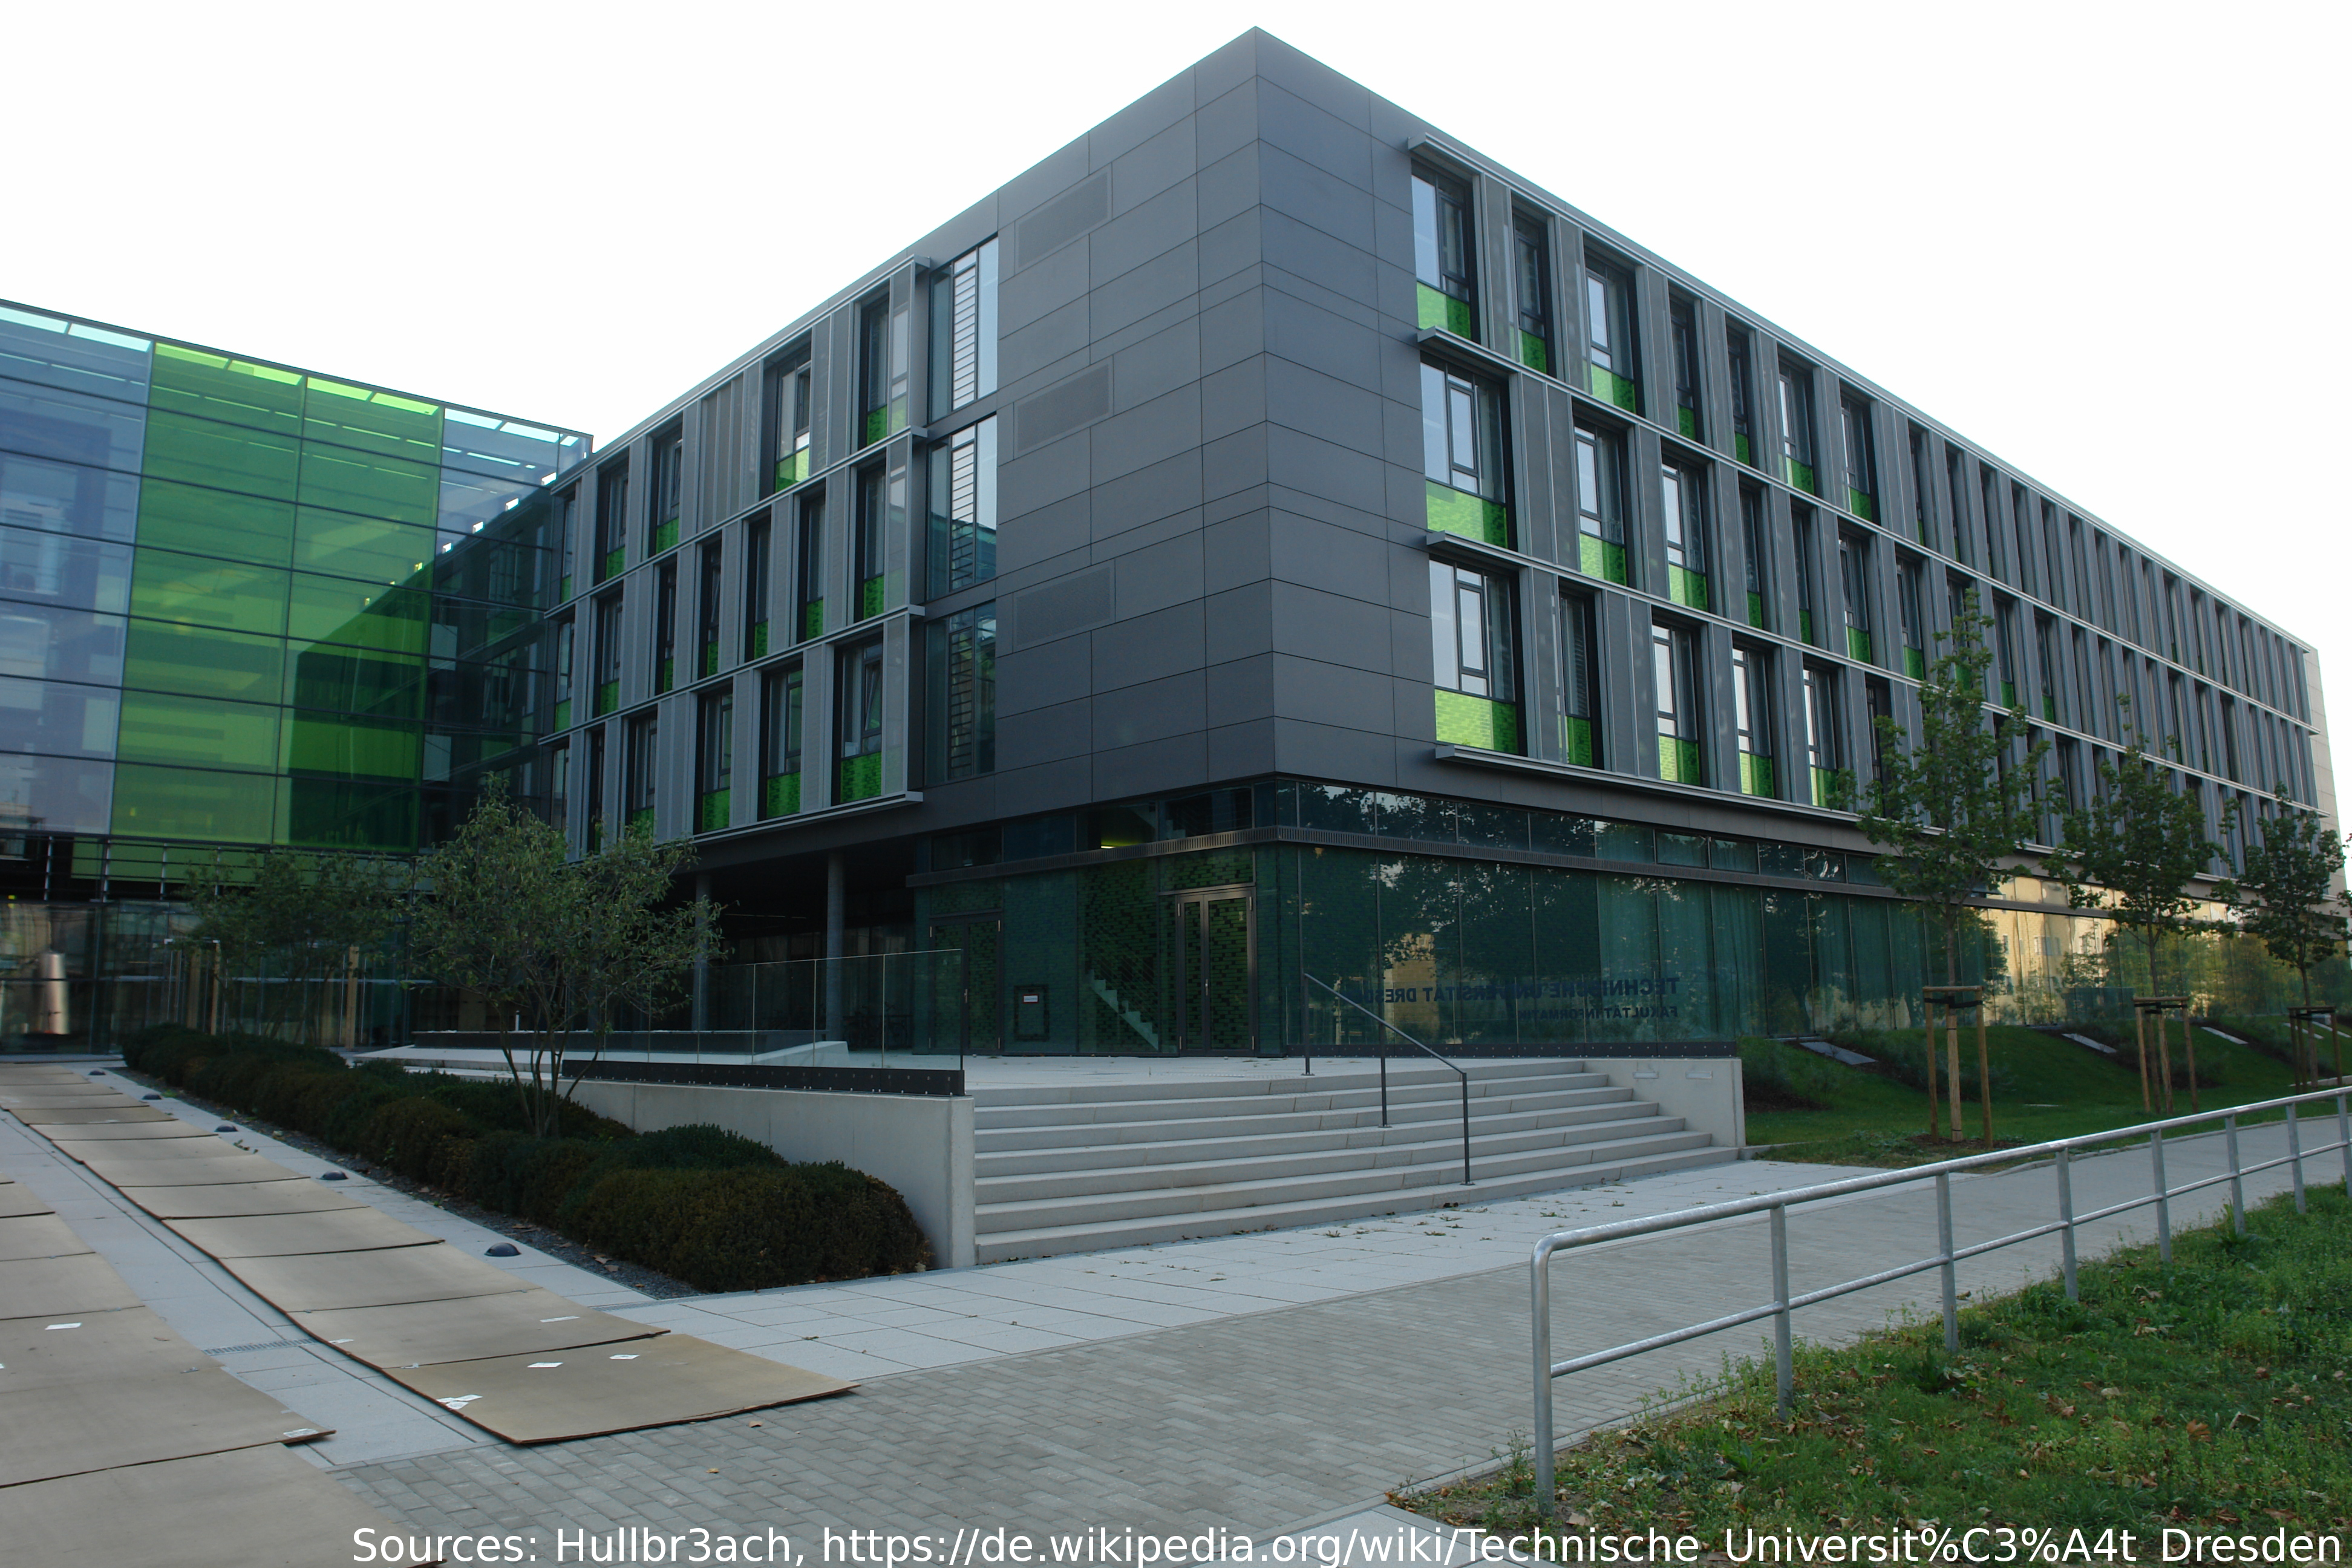
\includegraphics[width=1\linewidth]{images/informatik_bau.jpg}
\caption{Faculty of Computer Science building: Andreas-Pfitzmann-Bau.}
\label{informatik_bau}
\end{center}
\end{figure}

\subsection{Institute of Systems Architecture: Chair of Systems Engineering}

I was working in the Faculty of Computer Science under the Chair of Systems Engineering at the Institute of Systems Architecture. The following sections gives you more details about this chair.

\subsubsection{Head of the chair: Prof. Dr. Christof Fetzer}

The head of the chair is Prof. Dr. Christof Fetzer, as for the university I will not paraphrase so here is a quote from the university website \cite{tud:chair:head} regarding his background:

\blockquote{Christof Fetzer received his Ph.D. from UC San Diego (1997). 
As a student he received a two-year scholarship from the DAAD and won two best student paper awards (SRDS and DSN). 

He was a finalist of the 1998 Council of Graduate Schools/UMI distinguished dissertation award and won an IEE mather premium in 1999. Dr. Fetzer joined AT\&T Labs-Research in August 1999 and was a principal member of technical staff until March 2004. 

Since April 2004, he is head of the Systems Engineering Chair in the Computer Science Department at the Dresden University of Technology. He is the chair of the Distributed Systems Engineering International Masters Program at the Computer Science Department. Prof. 

Dr. Fetzer has published over 130 research papers in the field of dependable systems.}
 
\subsubsection{Fields of study}

This chair's fields of study are:
\begin{itemize}
\item
Fault tolerance
\item
Secure Cloud Application
\item
Stream Processing
\item
Parallel and distributed systems in general
\end{itemize}

I will follow an Engineering of Cloud Computing specialization for my third and last engineering year, so I was glad to be able to discover a few notions in advance like cluster computing systems as Apache Spark.

\subsubsection{What do they do?}

Their main project is SERECA --- Secure Enclaves for REactive Cloud Applications --- which is proposing a solution to secure cloud computing environment. Indeed, the adoption of cloud computing in Europe is slowed down by a lack of security guarantees \cite{tud:chair:project}.

They also do research on fields like Fault Tolerance \cite{tud:chair:papers:fault}, Event Stream Processing \cite{ tud:chair:papers:stream} and so on.

\subsection{Working environment}\label{working_environment}

People that I encountered were welcoming and interested in the work I did there. They did not hesitate to help me through my work by discussing some dark points even if they were not part of my team. Their feedbacks on features and inputs on some of my problems were essential.

The workstation provided by the university was perfect, I had strong personal machines that I could use without any restriction. This "liberal" working environment is crucial for me when developing applications. For example, system administration restrictions could be a large obstacle to quick development and progress.


\section{Internship benefits}

This internship helped me discover the research environment. It was interesting to realize that a PhD. student work was not quite as expected before working there. It is more a time management work divided into handle lecture exercises, side work like chair projects and last but not least your actual research work.

I think it would be an interesting place to work as it is different from a company working atmosphere. Despite a colorful and pleasant environment, I wish to continue my career by some company years before. 

I'm still interested in a PhD. but I think I lack of company experiences at the moment and I spend too much years of my life in school and universities. We all need some changes at a given moment.

\clearpage

\chapter{YCSB Web Interface visualization}

\section{Project organization}

\subsection{Team}

My supervisor --- Robert Krahn --- was the only person I actually work with. Nonetheless, people from the chair were also there to discuss ideas as I said in \ref{working_environment}. His inputs were crucial and he assisted me for decisive choices. He also guided me through the realization of this project as he will be one of its first user.

Robert presented me the purpose of the application and features I needed to implement as an extension module of Yahoo! Cloud Serving Benchmark code base. We refined these specifications over the development to make it suits future users needs.

\subsection{Working method}\label{working_method}

We used an AGILE like method to develop this project. As I was working alone on the implementation side, I needed to confront my features quickly to future users in order to get feedbacks.
The development cycle was simple. I began with a strong implementation phase followed by a testing and debugging phase. Then we used our tools to evaluate the solution and judge if it was suitable according to the expectations and use cases.

For example, at the end of the first cycle, our application was working great for small datasets but was crashing both on server and client side when it needed to handle thousands of points.
So, we made a complete review of the code to find bottlenecks and fixed them one by one like MongoDB aggregation, removal of useless layers, etc. We will elaborate on these optimizations in \ref{techical_chapter}.

\section{Application specifications}

The aim of this section is not to cover technical details but to explain in an accessible way what our application is offering. For more technical details, please go to \ref{techical_chapter}.

\subsection{Purpose of the application}

\subsubsection{Yahoo! Cloud Serving Benchmark}\label{ycsb}

As introduce beforehand, Yahoo! Cloud Serving Benchmark is used to evaluate performance of "key-value" and "cloud" serving stores. But how does it actually work?

The user defines a custom workload --- set of parameters which define how the benchmark will be executed --- or chose to use an existing one. Then, he starts the database he wants to benchmark and first launches YCSB \texttt{load} phase to fill the database with values --- INSERT operations. Finally he launches the \texttt{run} phase that executes operations --- READ, UPDATE, SCAN operations --- on the previously inserted values. All settings regarding proportions and quantity of these operations are defined in the workload file.

YCSB work is to store each CRUD operation execution time --- called \texttt{latency}. It provides measurement results --- \texttt{latencies} --- of the operations made during both \texttt{load} and \texttt{run} phase at the end of each phase.

YCSB has different way of displaying results, the most simple way is the RAW measurement type made by Google\footnote{Google RAW measurement type source code: \url{https://github.com/brianfrankcooper/YCSB/blob/master/core/src/main/java/com/yahoo/ycsb/measurements/OneMeasurementRaw.java}} as it simply displays a list of operations alongside with timestamps and latency results for each operation. Other measurement types exist and provide more information like quantiles or reducing precision to make results easier to read as timeseries' average buckets.

\subsubsection{What is the goal of our module and application?}

As you might have understood, YCSB is only producing results at the end of the execution process. If you want to perform a long benchmark that will run for hours, you might want to be able to watch final results fragments before the end of YCSB execution.

\bigskip

Our work was to make results available in a pseudo real-time --- low latency --- fashion without slowing YCSB performance. This last part is crucial: we must not slow YCSB in a non-acceptable manner.

There is no point of making a low latency result provider if there is no tool to visualize it. So we needed to implement a visualizer and we chose to implement a cool web interface that has pretty and convenient charts.

\subsection{General implementation ideas}

\subsubsection{YCSB extension module}

Providing low latency results to the user is achieved by storing measurements periodically into a storage database. This is the job of our YCSB extension module. The fetch of measures must be efficient and not disturbing for YCSB ongoing measurements.

\subsubsection{Web visualization}

Our web visualization is fetching the storage database measures and processing it to provide pretty and dynamic charts.

\clearpage

\chapter{Technical details}\label{techical_chapter}

Before the beginning of this chapter, we would like to inform you that two \texttt{README.md} files are available for both the visualization application and the YCSB extension module. They have valuable information about application parameters, tweaks and so on. We deeply encourage you to consult these files at the end of this chapter if you want more details as some parts will not be presented in this report.

\section{Application architecture}\label{app_archi_section}

The proposed solution architecture is made of two major parts that could operate separately. We have a software module that stores measures into the storage database and a visualizer application that displays these measures.

\begin{figure}[ht]
\begin{center}
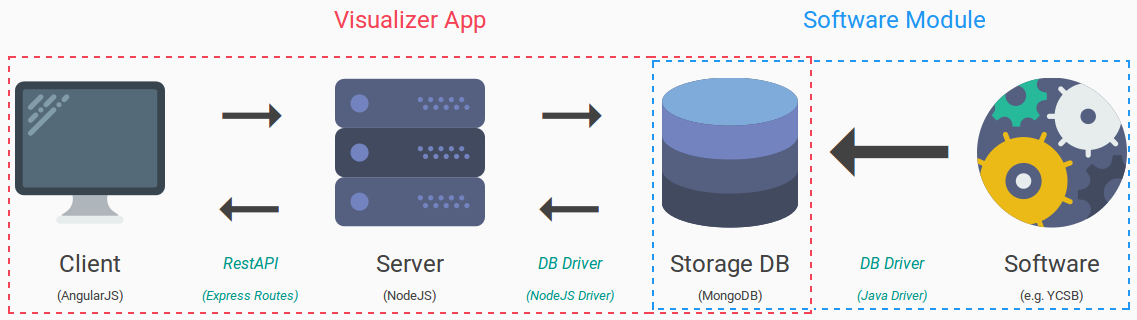
\includegraphics[width=1\linewidth]{images/archi_small_complete.png}
\caption{Application architecture visual.}
\label{app_archi_fig}
\end{center}
\end{figure}

You can see on Figure \ref{app_archi_fig} the different application modules and technologies that we used, AngularJS, NodeJS, MongoDB, etc. We will elaborate on our technology choices when describing each module in section \ref{technical_description}. 

\subsection{Architectural choices}

At first, we wished to expose a RestAPI directly from the YCSB Java application with technologies like Hazelcast. Sadly, it was drastically slowing the warm-up phase of YCSB so we tried a lightweight solution with ActiveJDBC and Spark Java --- not to be confused with Apache Spark --- and even this lightweight solution was slowing YCSB too much. 

Moreover, it forces the user to let YCSB running in the back even if no benchmark was launch thus the application modularity was not good enough for the maintainability of the solution. 

We realized that the performance reduction was inherent to the solution we proposed, we tried to bundle our solution too much. So we finally decided to let a MongoDB storage database be our "API" between the YCSB application and our web server. The database connection is quicker thus has a reduced impact on the warm-up phase compared to the former solutions. Also, the modularity provided by the storage DB allows our client/server application to communicate with \textit{every software capable of storing data into a MongoDB database}.

\section{Solution features}\label{technical_description}

\subsection{Software Module}

As mention in section \ref{app_archi_section}, the software module has to store the software measures into the storage database. In our case, our software was YCSB so we needed to extend YCSB functionalities to achieve a real-time storage of its measurements. 

Here, we will explain how the fetching process works and how does it stores measures into the storage database.

\subsubsection{Frontend MeasurementType}\label{concurrent_map_explainations} To achieve a better fetch of measures, we created a specific measurement type in YCSB. It is close to the raw measurement type --- explained in \ref{ycsb} --- as it stores all data without any processing before or after the storage. Our collection where we temporary stores values is an extended \texttt{ConcurrentMap}. Indeed, the YCSB client threads will write into the collection at the same time that we read it to fetch measures so we need that concurrent aspect.

\paragraph{How does this measurement type works ?}  Our \texttt{ConcurrentMap} is a map of fixed size lists of BSON Documents as we are working with a MongoDB storage database. When a new value needs to be stored, the map stores it into the current list, if this list is full it creates a new list and the latter becomes the current one. We have two integers that stores the id of the currently filled list and the last inserted list into the storage database. Do not worry, we have made a cool diagram (Figure \ref{concurrent_map_scheme}) to summarize all this for you.

\subsubsection{Fetching method}

We created a new thread into YCSB, indeed this is the most efficient way not to slow down YCSB too much. We used a scheduled thread pool executor of Java with only one thread. This scheduled executor thread periodically check the two integers of each \texttt{ConcurrentMap} --- one by client thread by operation type due to YCSB way of handling measures. These indicates which lists are available --- full and not designated as the current list --- without scanning the whole or even a part of our collection. 

Then, all available lists are processed into the executor thread to be stored into the storage database. Once a list has been stored, it is deleted from the \texttt{ConcurrentMap} in order to save some memory which is interesting with millions points benchmarks. This delete phase is not shown in Figure \ref{concurrent_map_scheme} for understanding purpose.


\paragraph{Fail-safe system}

There is two identical tasks that handles this fetching process and relaunch themselves after finishing their fetch. If one task fails, there is a fail-safe process that periodically relaunches a task if less than two fetching tasks are in the queue or running. At the end of the benchmark, all tasks are interrupted and a final task is run to fetch all remaining points --- even in the current list as the benchmark is done.

\subsubsection{Summary diagram}

We summarized the fetching process with an example that shows the \texttt{ConcurrentMap} states through a YCSB benchmark on Figure \ref{concurrent_map_scheme}.

\begin{figure}[ht]
\begin{center}
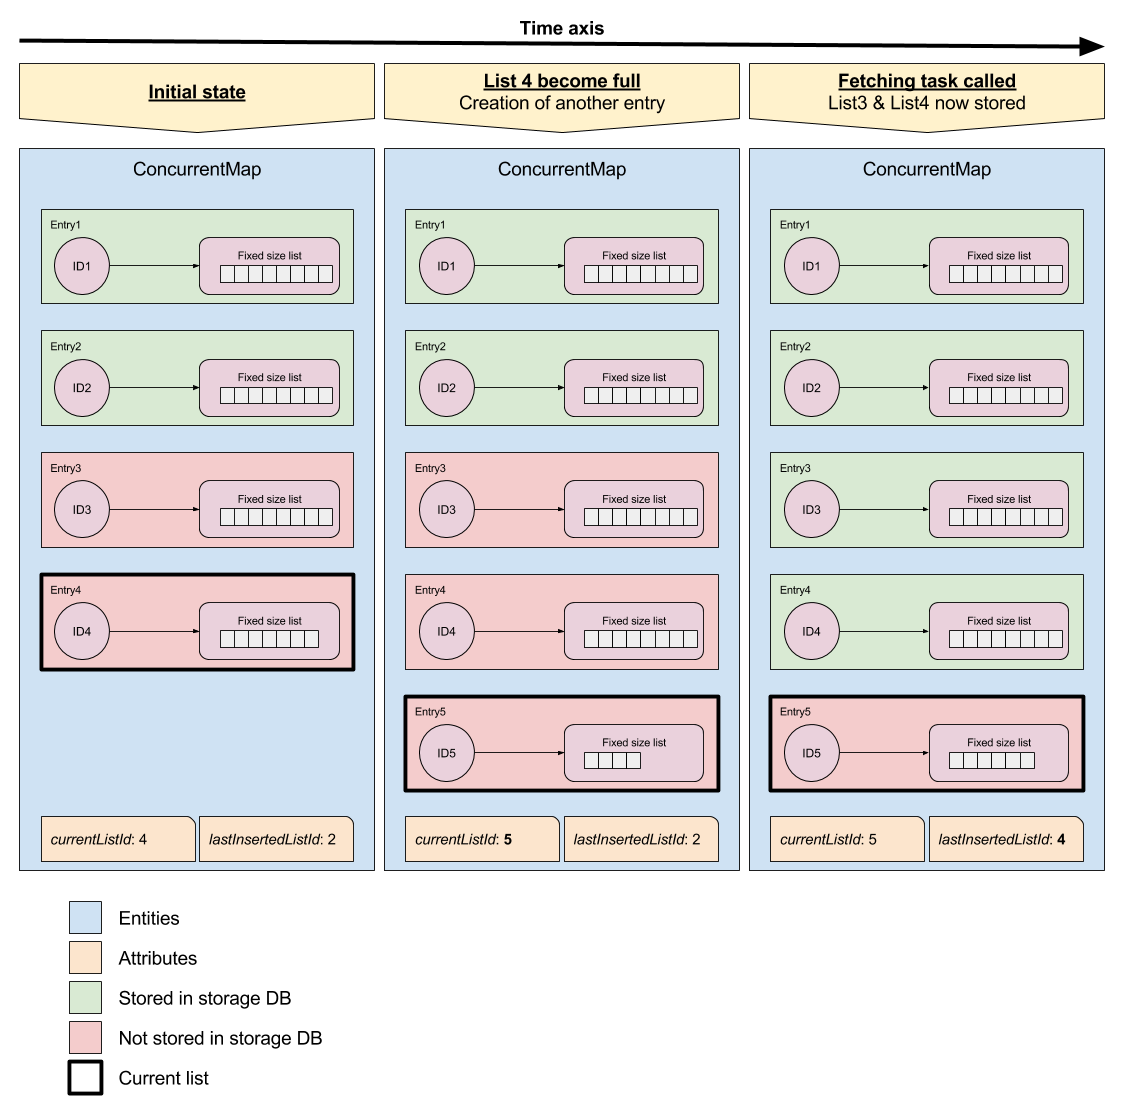
\includegraphics[width=1\linewidth]{images/concurrent_map_scheme.png}
\caption{\texttt{ConcurrentMap} states through a YCSB benchmark.}
\label{concurrent_map_scheme}
\end{center}
\end{figure}

\subsubsection{Communication with the storage database}

Only one connection is established with our MongoDB storage database in the executor thread. We used the native driver of MongoDB and unordered BULK writes for efficiency in insertion.

Indeed, as we had a large amount of measures to store at the same time on only one collection, we could use the performance advantage of a BULK write. Also, as we used a number to identify the order of our documents, we did not need to store them in an ordered fashion. This is much more efficient as MongoDB has full control on the insertions and makes the right performance choice regarding order. 

As lists are filled with BSON Documents, we did not have to do any processing before the insertion which is also a performance gain. 

\bigskip

We could have used the asynchronous driver or a larger pool of executor but we did not due to a lack of time evaluating this solution.

\subsection{Visualizer Application}

Again, as mention in section \ref{app_archi_section}, the visualizer application part is made to display measures that have been stored into the storage database. In our case, we displayed YCSB results. 

Here, we will elaborate on the purpose of each of our architecture module and explain why we chose these technologies.

\subsubsection{Implemented features}

\paragraph{Chart features}

Charts are automatically and periodically updating their points based on the storage database content. You only have to define which operation and type of chart you want to show and the chart will be initialized and updated over the time. We organize our views by benchmark --- identified by an unique name.

On top of this, Highcharts library \cite{highcharts:website} provides us a large set of interesting features. 
The navigator is useful to zoom and get a precise view of our dataset as you can see on Figure \ref{chart_not_zoomed_zoomed}. 
Moreover, chart axes are automatically adjusting regarding of the data it displays which is convenient. 

Charts are exportable into SVG image, CSV file of the whole series by a database dump or CSV file of the currently displayed series --- including averages. It can be useful to include results into documents as you can see on Figure \ref{chart_exportation}.

The chart view generates two average series each based on:
\begin{itemize}
\item
points of the whole series (in black on Figure \ref{chart_not_zoomed_zoomed})
\item
points currently displayed --- current navigator window (in green on Figure \ref{chart_not_zoomed_zoomed})
\end{itemize}

These lines are available for line charts only and can be disabled in the code with a simple parameter\footnote{Please consult the README.md file of the visualization application for more information}.

\begin{figure}[ht]
\begin{center}
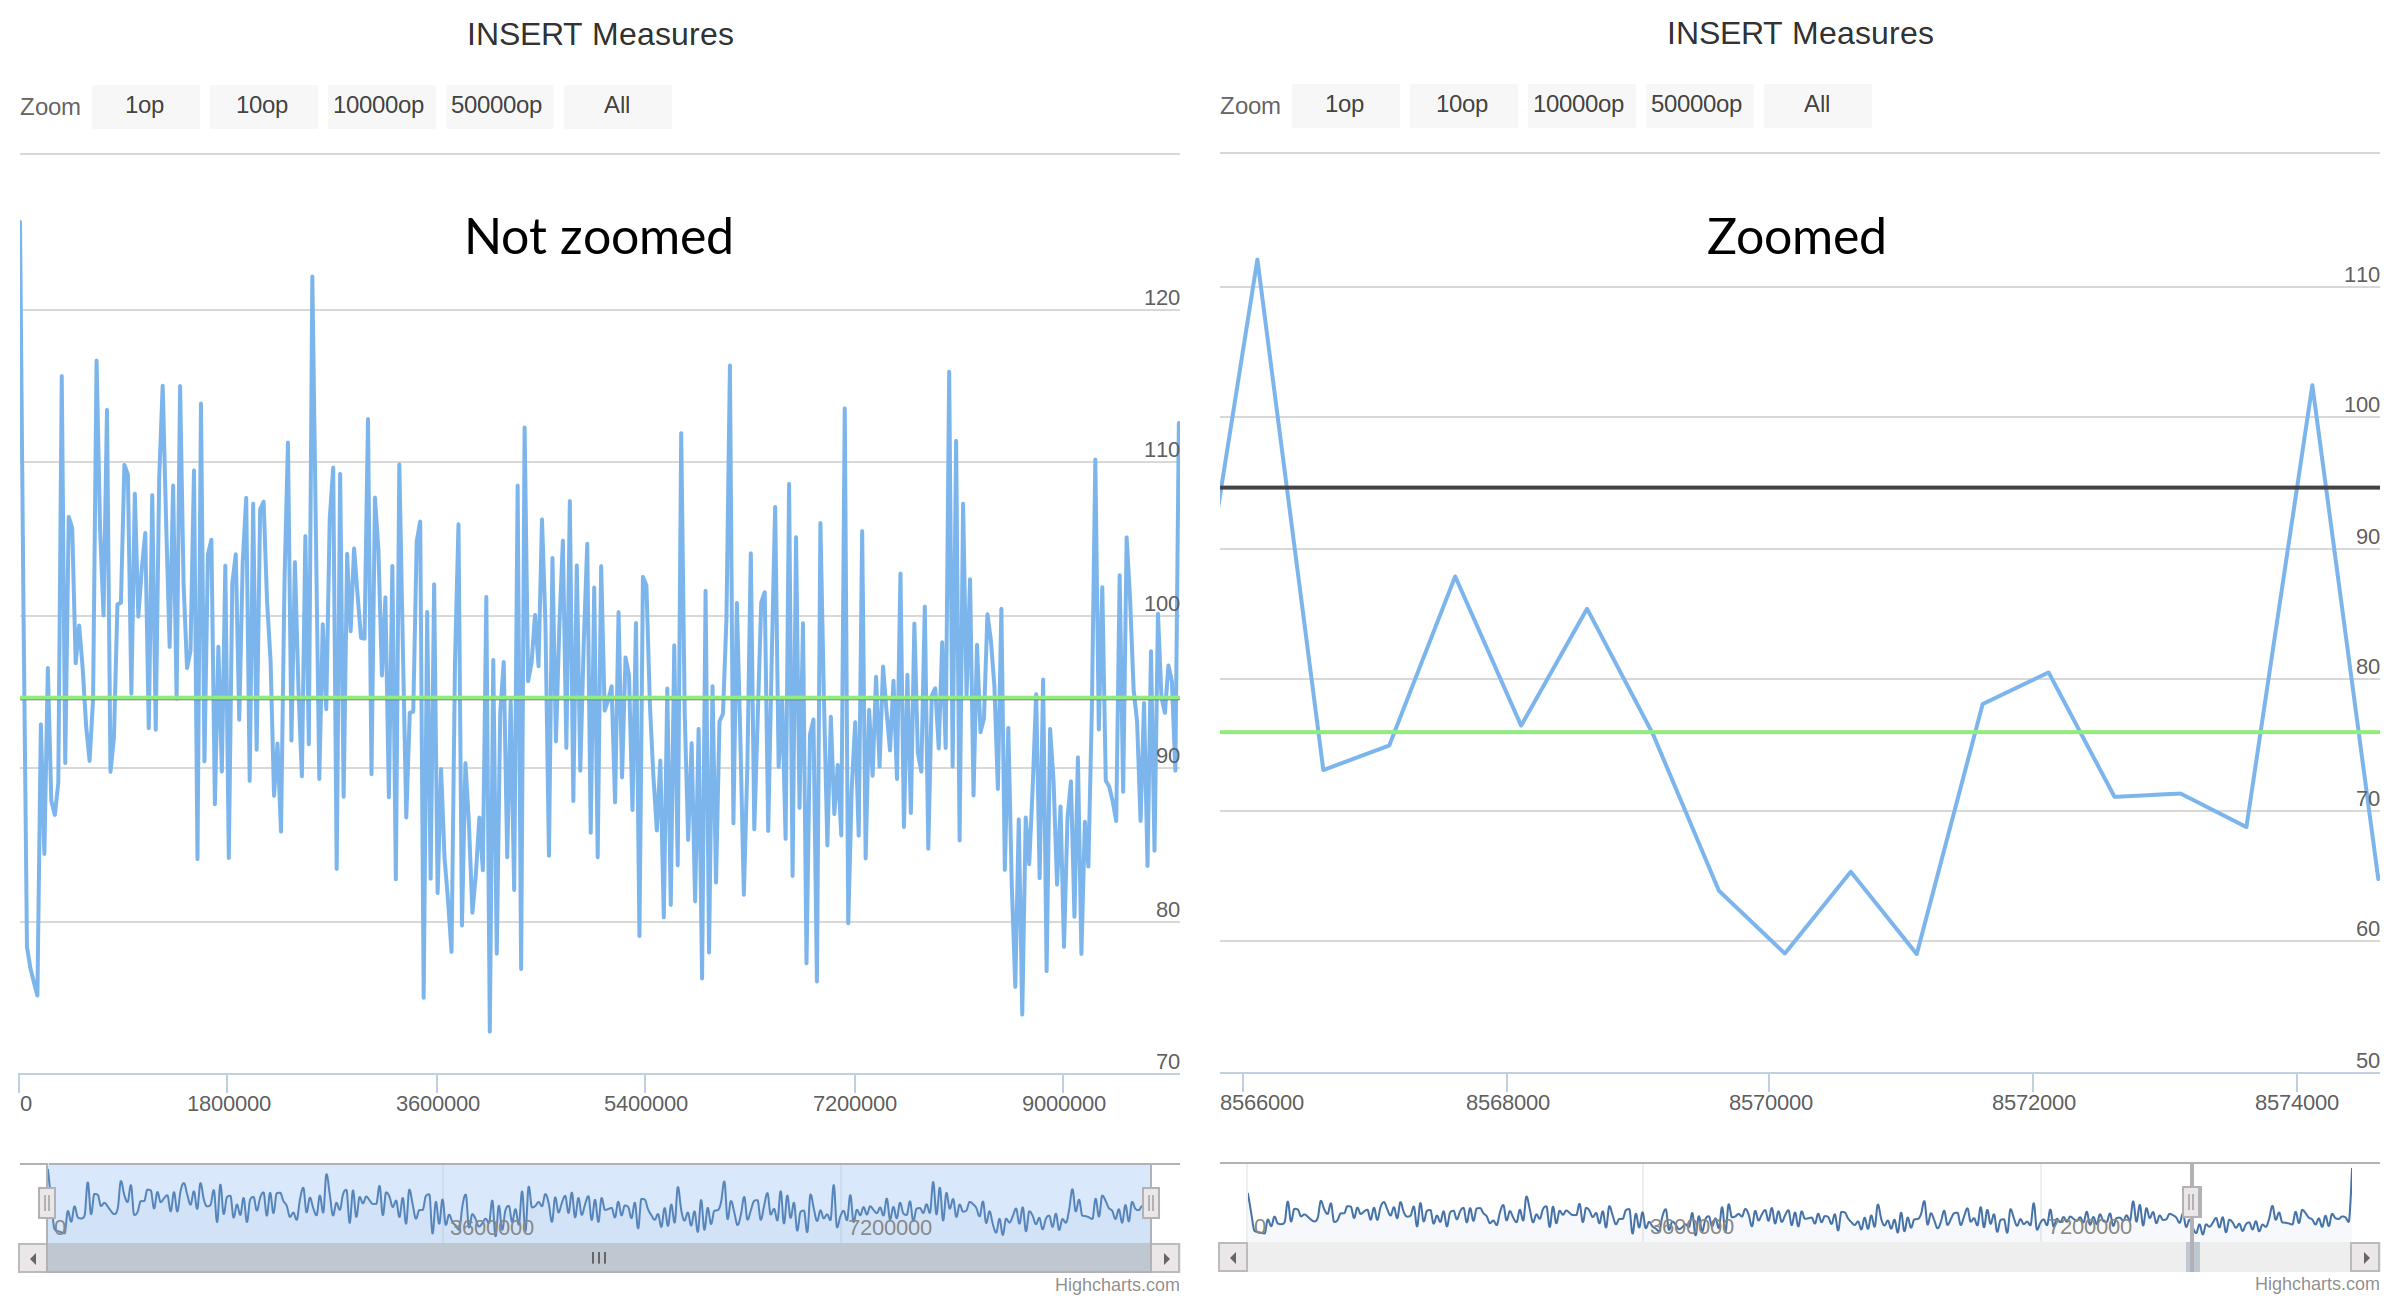
\includegraphics[width=1\linewidth]{images/chart_not_zoomed_zoomed.png}
\caption{Navigator functionality: zoom comparison.}
\label{chart_not_zoomed_zoomed}
\end{center}
\end{figure}

\begin{figure}[ht]
\begin{center}
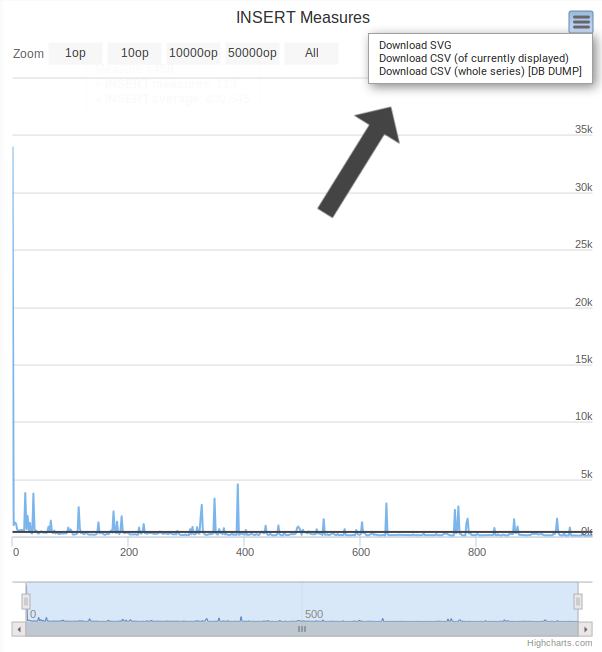
\includegraphics[width=0.6\linewidth]{images/chart_exportation.png}
\caption{Exportation functionality: dropdown menu.}
\label{chart_exportation}
\end{center}
\end{figure}
\clearpage
\subparagraph{YCSB warm-up phase suppressor}

During our experimentation, we noticed YCSB warm-up phase was drastically altering the average as the first operation latency measure includes the warm-up phase duration. We recommend that YCSB users remove the first point of their results if they want an cleaned average. The chart navigator can be used to do so by shrinking the window to remove the first point. The current window average line will then indicate an adjusted average that reflects the overall latency of the benchmark better.

\paragraph{Better than a simple visualizer for YCSB}

\subparagraph{YCSB benchmark launcher}

We implemented a benchmark launcher view to easily start YCSB benchmark from our web application. You can choose your benchmark name, YCSB phase, client thread number, workload file, etc. and then launch your benchmark (See Figure \ref{launcher_ui}).

\begin{figure}[ht]
\begin{center}
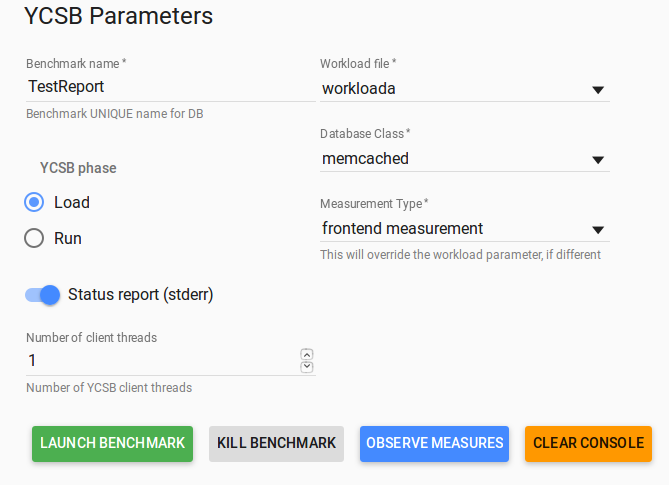
\includegraphics[width=1\linewidth]{images/launcher_ui.png}
\caption{Our benchmark launcher User Interface.}
\label{launcher_ui}
\end{center}
\end{figure}

We provide a standard output/error feedback (Figure \ref{cli_feedback}) thus the user interface launcher will not alter former users' experience as they will have YCSB console output information like they used to have.

\begin{figure}[ht]
\begin{center}
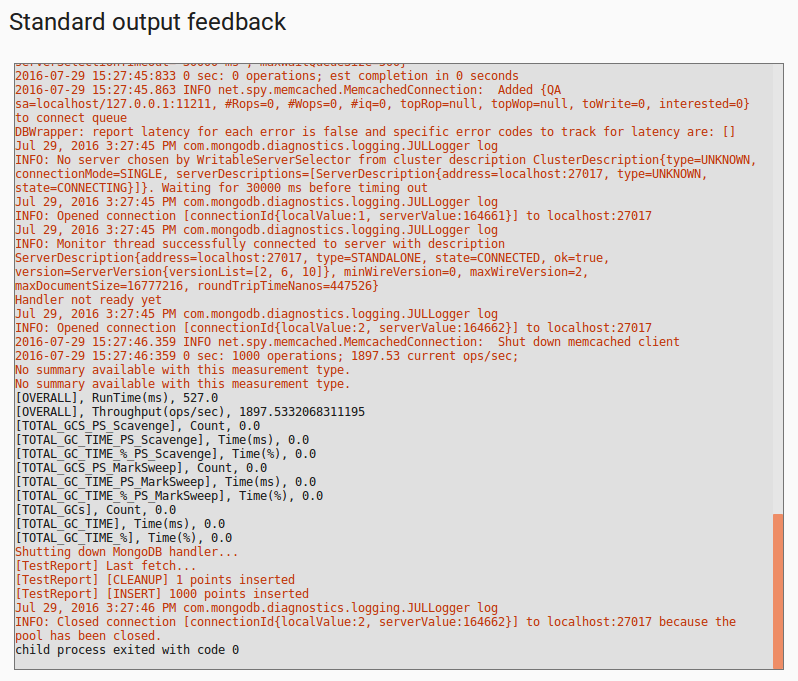
\includegraphics[width=1\linewidth]{images/cli_feedback.png}
\caption{Command Line Interface feedback within the web application.}
\label{cli_feedback}
\end{center}
\end{figure}

\bigskip

This interface is \textit{totally optional} and you can obviously use YCSB with its command line interface. The latter will work just as good as our launcher view with our visualizer.

This interface is specific to YCSB and does \textbf{not} support other benchmark software.

\subparagraph{Workload editor}

We also implemented a simple workload editor that save yourself wasting time by looking for your workloads file and edit them in your favorite text editor (See Figure \ref{workload_editor}).

\begin{figure}[ht]
\begin{center}
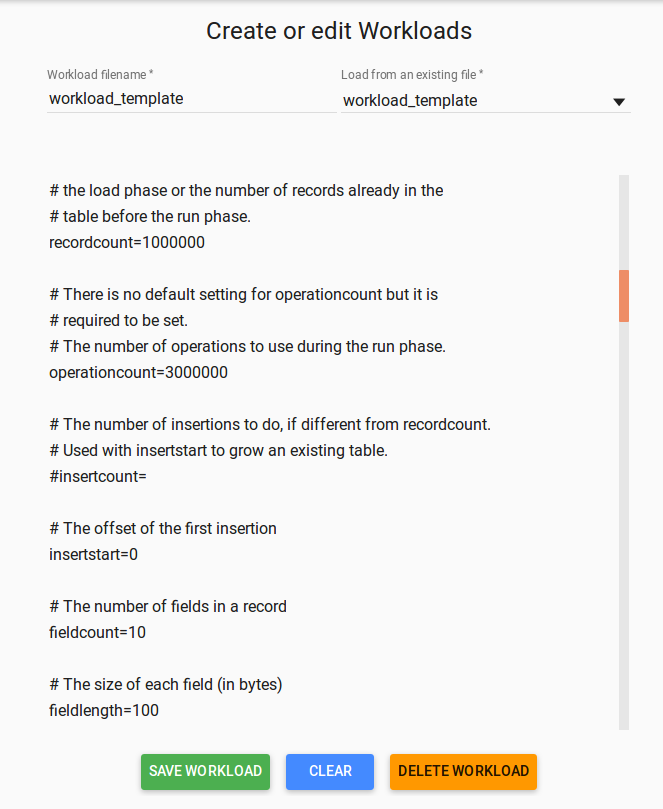
\includegraphics[width=0.8\linewidth]{images/workload_editor.png}
\caption{Simple workload editor.}
\label{workload_editor}
\end{center}
\end{figure}
\clearpage
\paragraph{Server role}

The main role of our server is to retrieve measures from the storage database and deliver them to the client. Furthermore, it handles the YCSB benchmark launch, provides the CLI feedback and executes file operations asked by the workload editor. 

\subsubsection{Server side technology choices}

We chose NodeJS because we needed a lightweight and easy to deploy server. NodeJS is perfect for this use case and can communicate easily with a MongoDB database as well as simply exposing a RestAPI and handling web-sockets.

\paragraph{Communication with Storage DB}\label{server:mongo}

We used the native NodeJS driver made by the MongoDB developers. We could have use the well known Mongoose ODM but our queries and server was so simple that we did not need to add this layer. Moreover, Mongoose is reducing performance as it add some logic layers between the code and the actual query execution or result \cite{mongo}.

\paragraph{Handling large datasets}\label{server:handling_large_dataset}

Our server is capable of handling multi-millions points benchmarks. We used MongoDB aggregation functions to do so.

When handling large datasets, NodeJS asks MongoDB to use aggregations to group measures by making averages thus optimize the view fluidity. This grouping process reduces measurements' precision. This loss is illustrated by the example on Figure \ref{mongo_agg}. In this example, you would get 3 average measures --- buckets --- each based on 3 successive values instead of getting 9 plain measures.

The limit between a large and small dataset is fixed by an user parameter called \texttt{MAX\_POINTS}. The better your computer and browser are, the higher you can set the value and the smaller the average buckets will be thus you will have a more precise dataset. Again, please consult the \texttt{README.md} file for more information.

\begin{figure}[ht]
\begin{center}
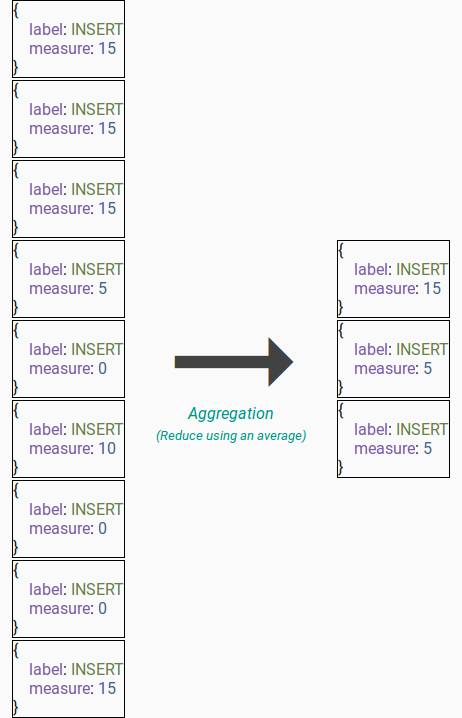
\includegraphics[scale=0.35]{images/mongodb-agg.png}
\caption{Simple illustration of MongoDB aggregation process.}
\label{mongo_agg}
\end{center}
\end{figure}

\clearpage

\subsubsection{Client side technology choices}

We develop our client with AngularJS because it is easy to maintain and forces a structured code base with a Model View Controller like pattern. Moreover, Angular provides helpful functionalities for forms, RestAPI communications, updates and dynamic behaviors of our application pages, etc. \cite{angular:website}.

\paragraph{Initialization \& update processes}

We made a custom directive for handling Highcharts charts generation based on the one provided by its developers. We added the initialization and update processes including an average calculation on top of this. These two processes simply modify Highcharts series with Highcharts API functions. Each chart gets its own initialization and update tasks.

These tasks check the current size of the benchmark to decide if a MongoDB aggregation must be made or not. If a MongoDB aggregation is needed, they define the bucket size --- the size of the group of points made by the aggregation. Finally, they query the right points based on these parameters and update their chart.

\paragraph{Highcharts library: data grouping}\label{data_grouping} There is plenty of chart libraries for web applications but Highcharts most valuable asset is its DataGrouping and that is why we chose it.

Indeed, Highcharts automatically groups points based on there proximity --- pixel wise --- and if you zoom in you will get your precision back as the chart will be repopulated by former missing points. It makes charts look great and readable as well as keeping the original precision.

We have then two optimizations for large dataset, Highcharts client side data grouping that reduces the number of points display on charts without loosing information and MongoDB server side aggregation process for larger benchmark that reduces precision of measurements a bit.

Moreover, this library provides easily "tweakable" graphs and that handles update properly. Highcharts developers also made possible the integration within Angular with a directive.

\paragraph{Angular Material} We used a style framework because we did not have plenty of time to spend making our application look good. Angular Material provides amazing features to quickly make responsive websites that look great.

\section{Increasing support}

\subsection{File import module}

We realized during the development of our extension module for YCSB that it was not made for tiny benchmark --- around 1k to 10k points. Indeed, it slows down YCSB to much in this case --- SPOILER ALERT... too late, sorry! We did not want to force YCSB users to wait because our module was slow on tiny benchmarks. So we made an import module on the web interface!

\paragraph{How does it work?}

YCSB users launch their tiny benchmarks without using our measurement type, for example they could use the RAW measurement type. This means launching YCSB the old way with a file insertion at the end. Then, they can visualize charts by importing their files into our web application (See Figure \ref{import_module})!

\begin{figure}[ht]
\begin{center}
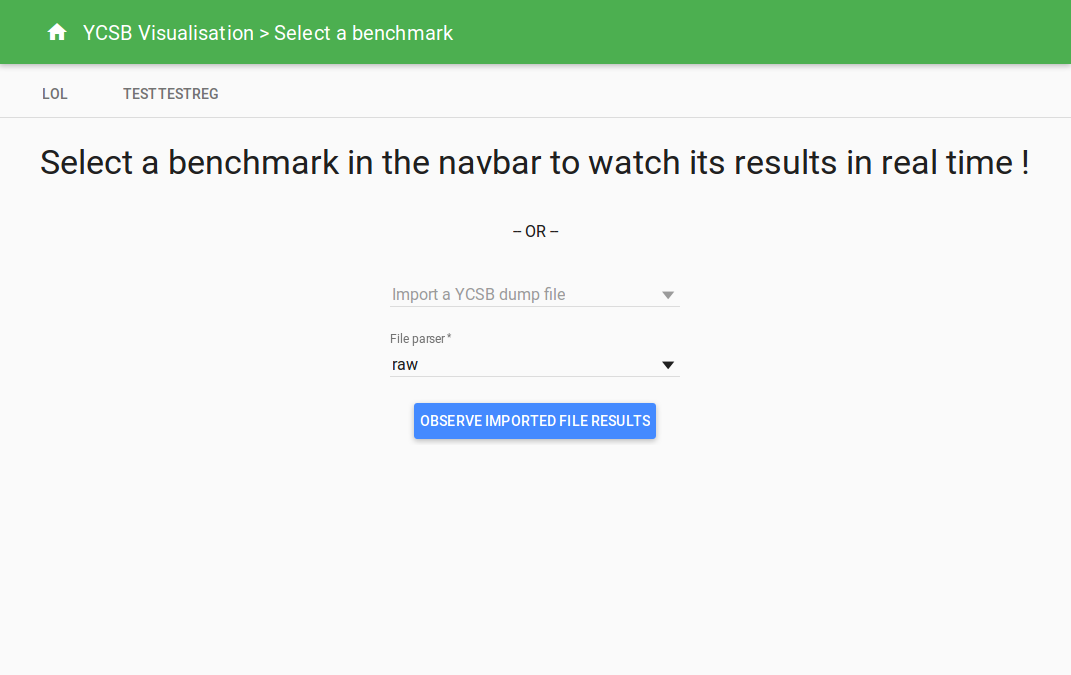
\includegraphics[scale=0.35]{images/import_module.png}
\caption{Import module location.}
\label{import_module}
\end{center}
\end{figure}

\paragraph{Limitations}

For now, the only measurement type that is supported by our import module is the RAW measurement type. However, it is simple to implement new parsers! For more information consult the \texttt{README.md} file of the visualization application.

The import module is not persistent! You will need to import your file each time you want to visualize them as they are not stored into the MongoDB database.
Also, it does obviously not support real-time updates.

\subsection{Other software than YCSB}

At first, the main idea was to provide a visualization web interface for YCSB benchmarks. Nonetheless, we realized that as we build this modular solution, we could support any software that could store data into a MongoDB database.

If you want to use a different software than YCSB, you need to respect the way we insert data into our storage database and our application would be automatically display your results. For more information consult the \texttt{README.md} file of the visualization application.

\subsection{Multiple chart types}

We also implement our chart view in a way that supporting multiple chart types is a child's play. Indeed, you just need to:

\begin{itemize}
\item
tell our application how you stored you data in the storage database
\item
tell our application how should Highcharts understand it
\item
which Highcharts chart type you wish to display
\end{itemize}

These three points are, in fact, trivial functions that are obvious and effortless to write. On the contrary, supporting large dataset with your custom type would be \textbf{a little bit harder} to do, depending on your chart type, because it would require some MongoDB aggregation understandings.

\subsubsection{Candlestick example}

We implemented candlestick --- boxplot without median --- charts support to prove our point and providing a solid example for the documentation. See Figure \ref{candlestick} to see the result!

Again, for more specific details of implementation, please consult the \texttt{README.md} file of the visualization application. It has a deeply detailed explanation of how to implement it.

\begin{figure}[ht]
\begin{center}
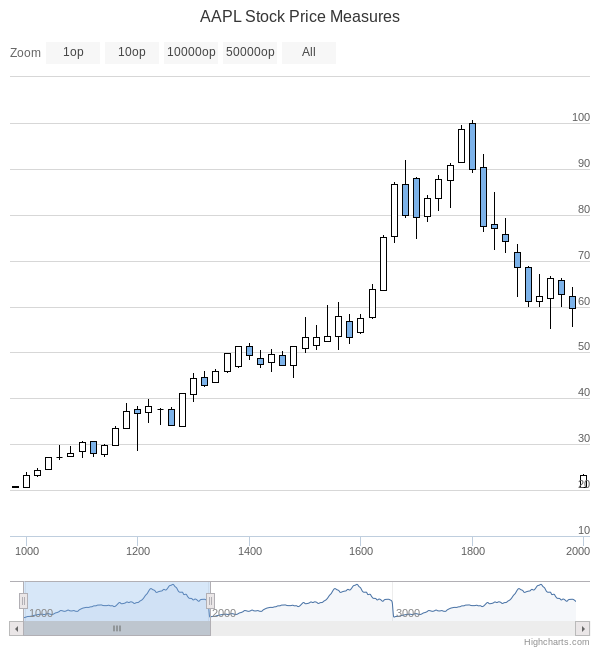
\includegraphics[scale=0.45]{images/candlestick.png}
\caption{Example of a candlestick chart.}
\label{candlestick}
\end{center}
\end{figure}

\chapter{Evaluation}

\section{Performances}

YCSB speed is based on the operation it can achieve by seconds --- ops/sec or \textit{Throughput}. The main challenge for our YCSB extension module was not to slow down the whole benchmarking process as we explained in previous chapters.

This evaluation will be comparing the RAW measurement type of Google and our custom measurement type that stores values into the storage database.

We will evaluate two indicators, the first one is the YCSB's \textit{Throughput} of a benchmark phase and the second one is the overall execution time of a benchmark phase. Indeed, this second parameter appears like an interesting comparison indicator of our module as our measurement type requires a database connexion and an additional thread.

\bigskip

This evaluation only purpose is to evaluate our extension module performances and not YCSB performances. We will \textbf{not} compare results between different operation proportions --- different workloads (A, B, C, etc.) --- as the process involved by this parameter change is identical in the two measurement types thus refer to a YCSB specific behavior.

However, we will compare the influence of remote or local state of both storage and benchmarked databases and the difference between a single and multi threaded YCSB benchmarking process. 

We will compare a major factor for the extension module measurement type: the number of points in the benchmark. We want to remind you that our module is made for large benchmarks and we do not expect it to work efficiently for small benchmarks.

\subsection{Before getting started}

\subsubsection{\textit{Throughput} efficiency evaluation point range reduction}

From 1k to 10k operations in the benchmark--- the size of our Concurrent Map lists, explained in \ref{concurrent_map_explainations} --- we observe unpredictable results because the fetch of the points will always occur at the end of the benchmark. This is really not a problem as our extension module is not made for small benchmarks. Nonetheless, users should keep in mind that they won't be able to predict the efficiency of our module when dealing with small benchmarks.

From 15k to 90k operations in the benchmark, we observe less but still dispersed results. It must be due to the fact that the benchmark is done right after the first iteration of our fetching process.

In both cases, initialization time is influenced by the Operating System of the YCSB host machine and is hard to grasp.

\textit{Throughput} efficiency evaluation will then not consider results below 90k points.

\subsubsection{How to understand our evaluation charts}

\paragraph{Y-Axis}

All the following charts have an "Efficiency" Y-Axis, it represents the influence of our measurement type on the efficiency of the RAW measurement type. For example, an efficiency of -2\% means that our measurement type for the same experiment --- same parameters --- is 2\% \textbf{slower} than the RAW measurement.

\paragraph{Legend} You will observe weird series names while watching our graphs. This notation is a convenient to know exactly the parameters of the series we are watching. Let us introduce you to this trivial notation:

\begin{itemize}
\item
I means \textit{Iterations}, \texttt{I20} means that the result have been obtained after $20*2$ iterations of couple of load and run phases of each configuration --- 20 iterations with the custom measurement type and 20 with the RAW measurement type
\item
M means \textit{Memcached}, \texttt{M10.0.0.3:11211} is a remote address of our \textbf{benchmarked} database, you will also see the famous \texttt{M127.0.0.1:11211} which is the local address obviously
\item
S means \textit{Storage}, \texttt{M10.0.0.3:27017} is a remote address of our \textbf{storage} database, you will also see the famous \texttt{S127.0.0.1:27017} which is the local address obviously
\item
T means \textit{Threads}, \texttt{T1} means that a single client thread is used.
\item
Sometimes you will see \texttt{median}, \texttt{average} or \texttt{boxplot} at the end, which indicates the series type ; this can be convenient when dealing with both average and median
\end{itemize}

\subsection{\textit{Throughput} efficiency}

\subsubsection{Remote/Local storage database}

\paragraph{Fixed parameters}
\begin{itemize}
\item
Range: 90k to 1M
\item
Remote benchmarked database
\item
Single threaded environment (1 client thread to limit side effects)
\end{itemize}

\paragraph{Results}

The following results of Figures \ref{storage-T1-Mremote-load}  \& \ref{storage-T1-Mremote-run} and Table \ref{storage-table} have been obtained after $20*2$ iterations of couple of load and run phases of each configuration --- 20 iterations with the custom measurement type and 20 with the RAW measurement type.

\begin{figure}[ht]
\begin{center}
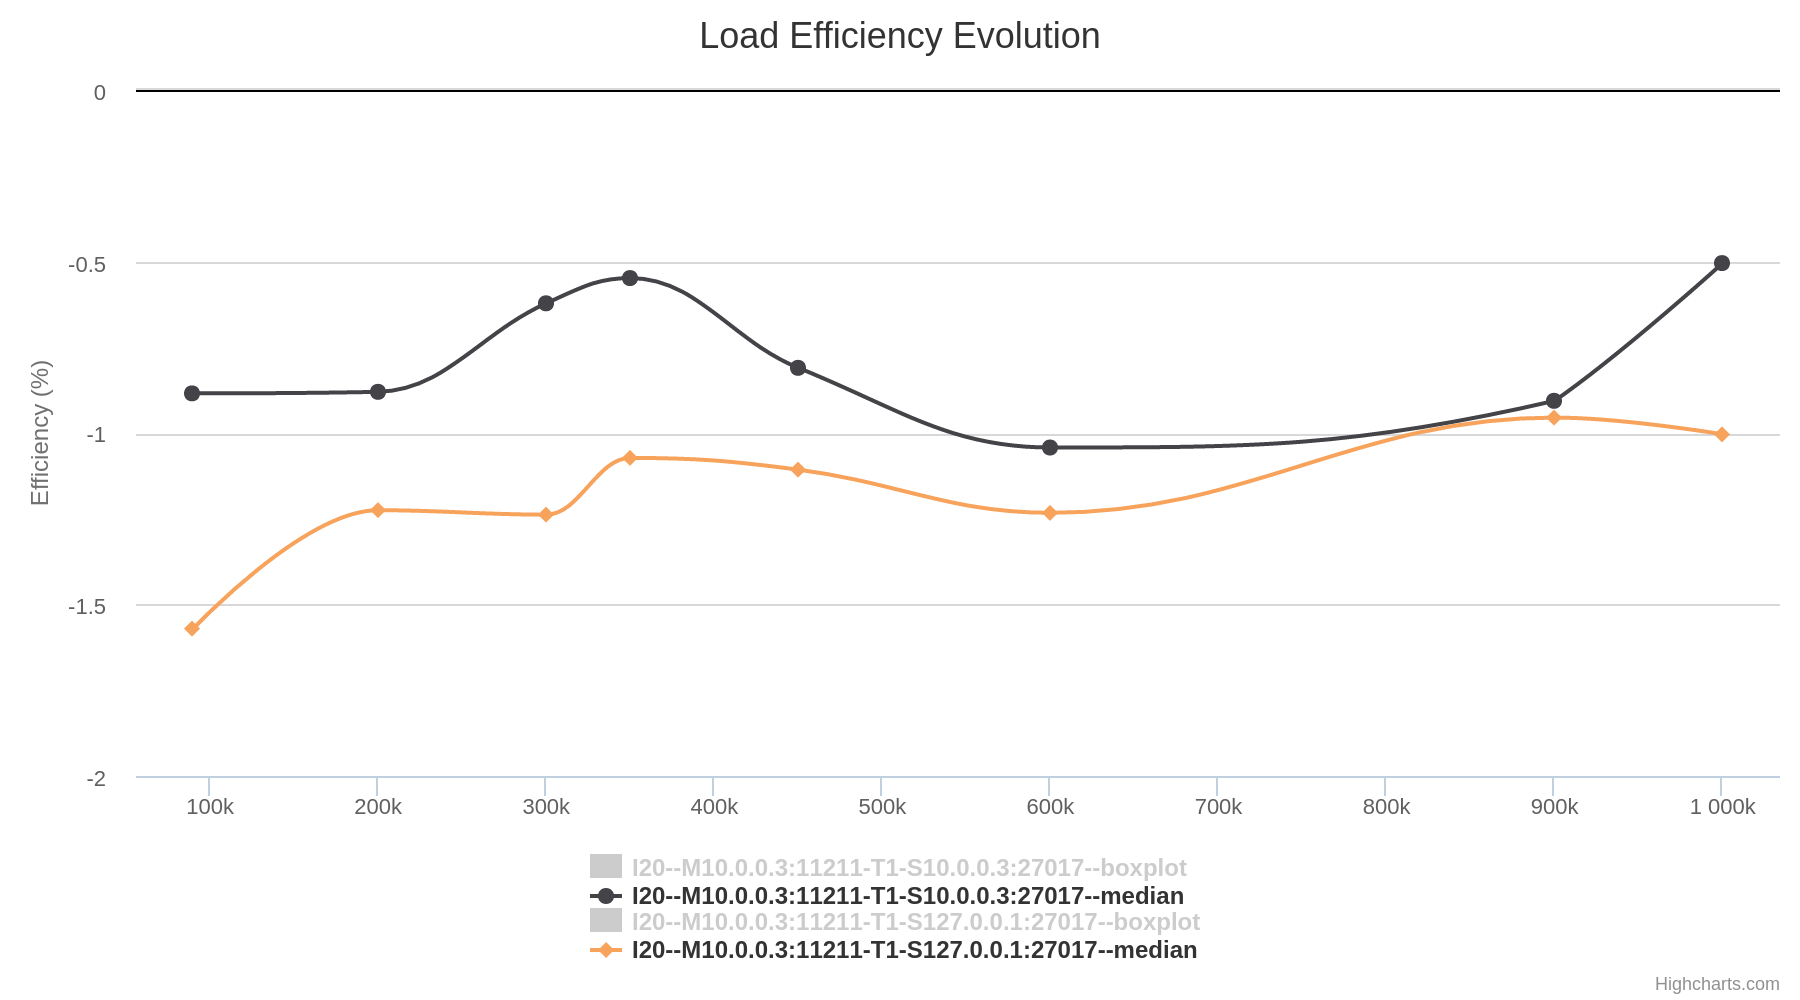
\includegraphics[width=1\linewidth]{images/evaluation/storage-T1-Mremote-load.png}
\caption{Storage database location comparison: load efficiency.}
\label{storage-T1-Mremote-load}
\end{center}
\end{figure}

\begin{figure}[ht]
\begin{center}
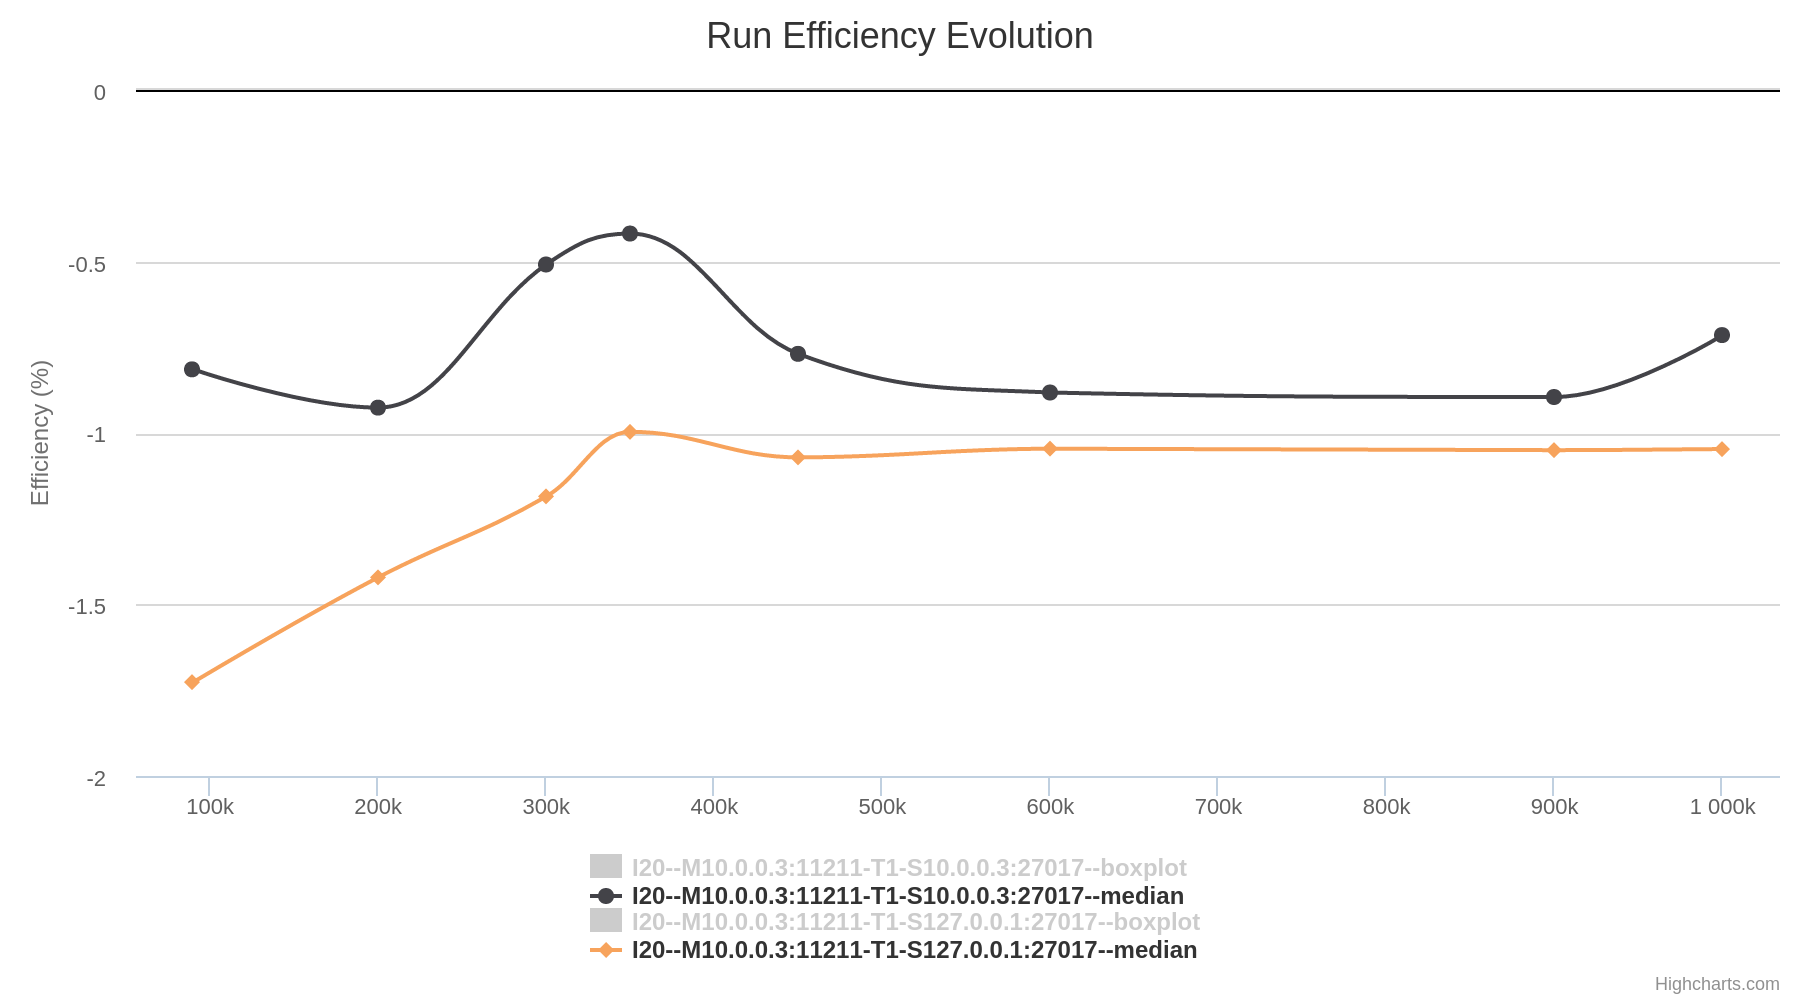
\includegraphics[width=1\linewidth]{images/evaluation/storage-T1-Mremote-run.png}
\caption{Storage database location comparison: run efficiency.}
\label{storage-T1-Mremote-run}
\end{center}
\end{figure}

\begin{table}[ht]
\begin{center}
	\begin{tabular}{|c|c|c|}
		\hline
		  & Local storage DB & Remote storage DB \\
		\hline
	   	LOAD phase & 0.5\% - 1\% slower & 1\% - 1.75\% slower \\
	   	RUN phase & 0.5\% - 1\% slower & 1\% - 1.75\% slower \\
	    \hline
	\end{tabular}
	\caption{Storage database location comparison.}
\label{storage-table}
\end{center}
\end{table}


\paragraph{Conclusion}

Having a remote storage database is more efficient according to the median because it uses less resources of the YCSB host machine. However, the location of the storage is not influencing the efficiency significantly as we have at most a difference of 1\%.

\clearpage

\subsubsection{Remote/Local benchmarked database}\label{memcached_evaluation}

\paragraph{Fixed parameters}
\begin{itemize}
\item
Range: 90k to 1M
\item
Remote storage database (results are quasi identical with a local one)
\item
Single threaded environment (1 client thread to limit side effects)
\end{itemize}


\paragraph{Results}

The following results of Figures \ref{benchmarked-T1-Sremote-load}  \& \ref{benchmarked-T1-Sremote-run} and Table \ref{benchmarked-table} have been obtained after $20*2$ iterations of couple of load and run phases of each configuration --- 20 iterations with the custom measurement type and 20 with the RAW measurement type.

\begin{figure}[ht]
\begin{center}
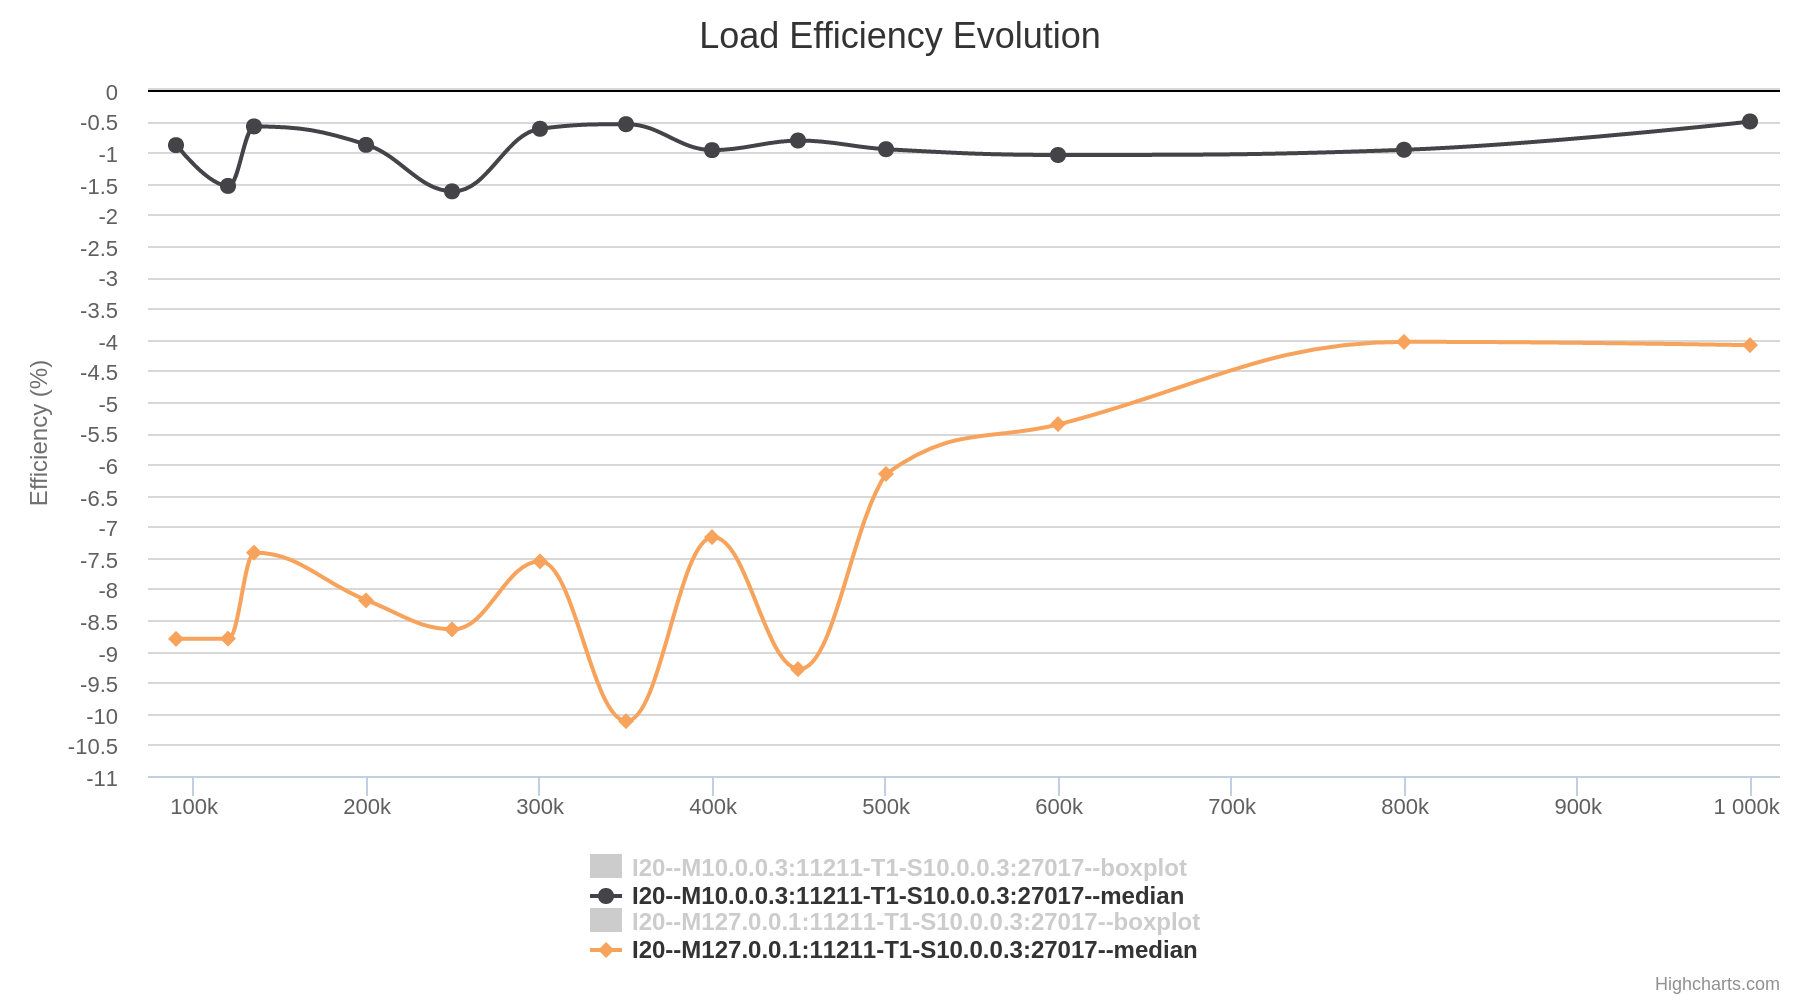
\includegraphics[width=1\linewidth]{images/evaluation/benchmarked-T1-Sremote-load.png}
\caption{Benchmarked database location comparison: load efficiency.}
\label{benchmarked-T1-Sremote-load}
\end{center}
\end{figure}

\begin{figure}[ht]
\begin{center}
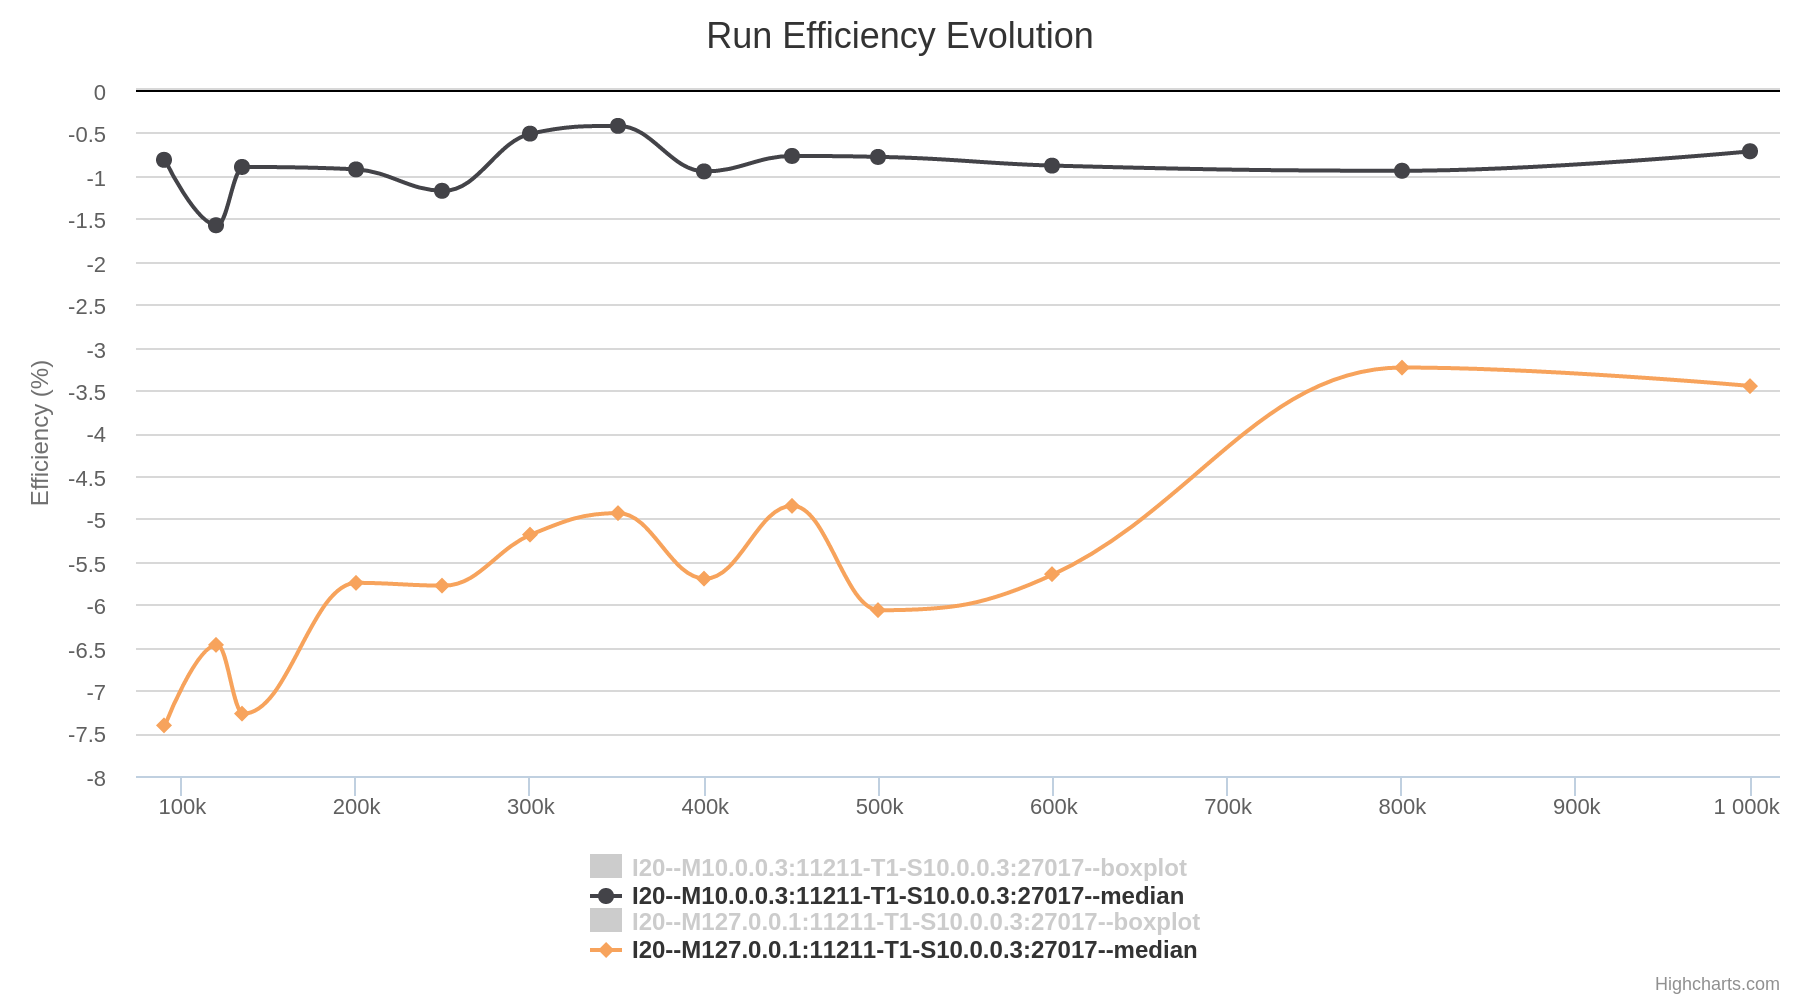
\includegraphics[width=1\linewidth]{images/evaluation/benchmarked-T1-Sremote-run.png}
\caption{Benchmarked database location comparison: run efficiency.}
\label{benchmarked-T1-Sremote-run}
\end{center}
\end{figure}

\begin{table}[ht]
\begin{center}
	\begin{tabular}{|c|c|c|}
		\hline
		  & Local benchmarked DB & Remote benchmarked DB \\
		\hline
	   	LOAD phase & 4\% - 10\% slower & 0.5\% - 1.5\% slower \\
	   	RUN phase & 3.25\% - 7.5\% slower & 0.5\% - 1.5\% slower \\
	    \hline
	\end{tabular}
	\caption{Benchmarked database location comparison.}
\label{benchmarked-table}
\end{center}
\end{table}

\paragraph{Conclusion}

We observe a huge difference in global efficiency. As you can see on the Figures \ref{benchmarked-T1-Sremote-load} \& \ref{benchmarked-T1-Sremote-run}, YCSB is slower when using a local benchmarked database than a remote one. YCSB is almost 9 time slower at worst (4 time slower at best) during LOAD phase and  7.5 time slower at worst (3 time slower at best) during RUN phase. 

In fact, having a remote benchmarked database is more efficient because it uses less resources of the YCSB host machine. Unlike the storage database, a benchmarked database is overused during a YCSB process \textbf{We invite users to use a remote benchmarked database for their benchmarks}. Moreover, this overload impact the stability in the result of local database, the local curve has a wider range than the remote one.

\clearpage

\subsubsection{Single/Multi threaded environment}

We need to be careful in conclusions in this section. Indeed, changing the number of client threads is a change that occurs on our measurement type but also in the RAW measurement type! Until now, modified parameters were only affected our measurement type. Here, we did not evaluate the advantage of using a single or multi threaded environment but we compare \textbf{how much our measurement type reduce the performance of both environment independently}.


\paragraph{Fixed parameters}
\begin{itemize}
\item
Range: 105k to 1M
\item
Remote storage database
\item
Remote benchmarked database
\end{itemize}


\paragraph{Results}

The following results of Figures \ref{thread-SMremote-load}  \& \ref{thread-SMremote-run} and Table \ref{thread-table} have been obtained after $20*2$ iterations of couple of load and run phases of each configuration --- 20 iterations with the custom measurement type and 20 with the RAW measurement type.

\begin{figure}[ht]
\begin{center}
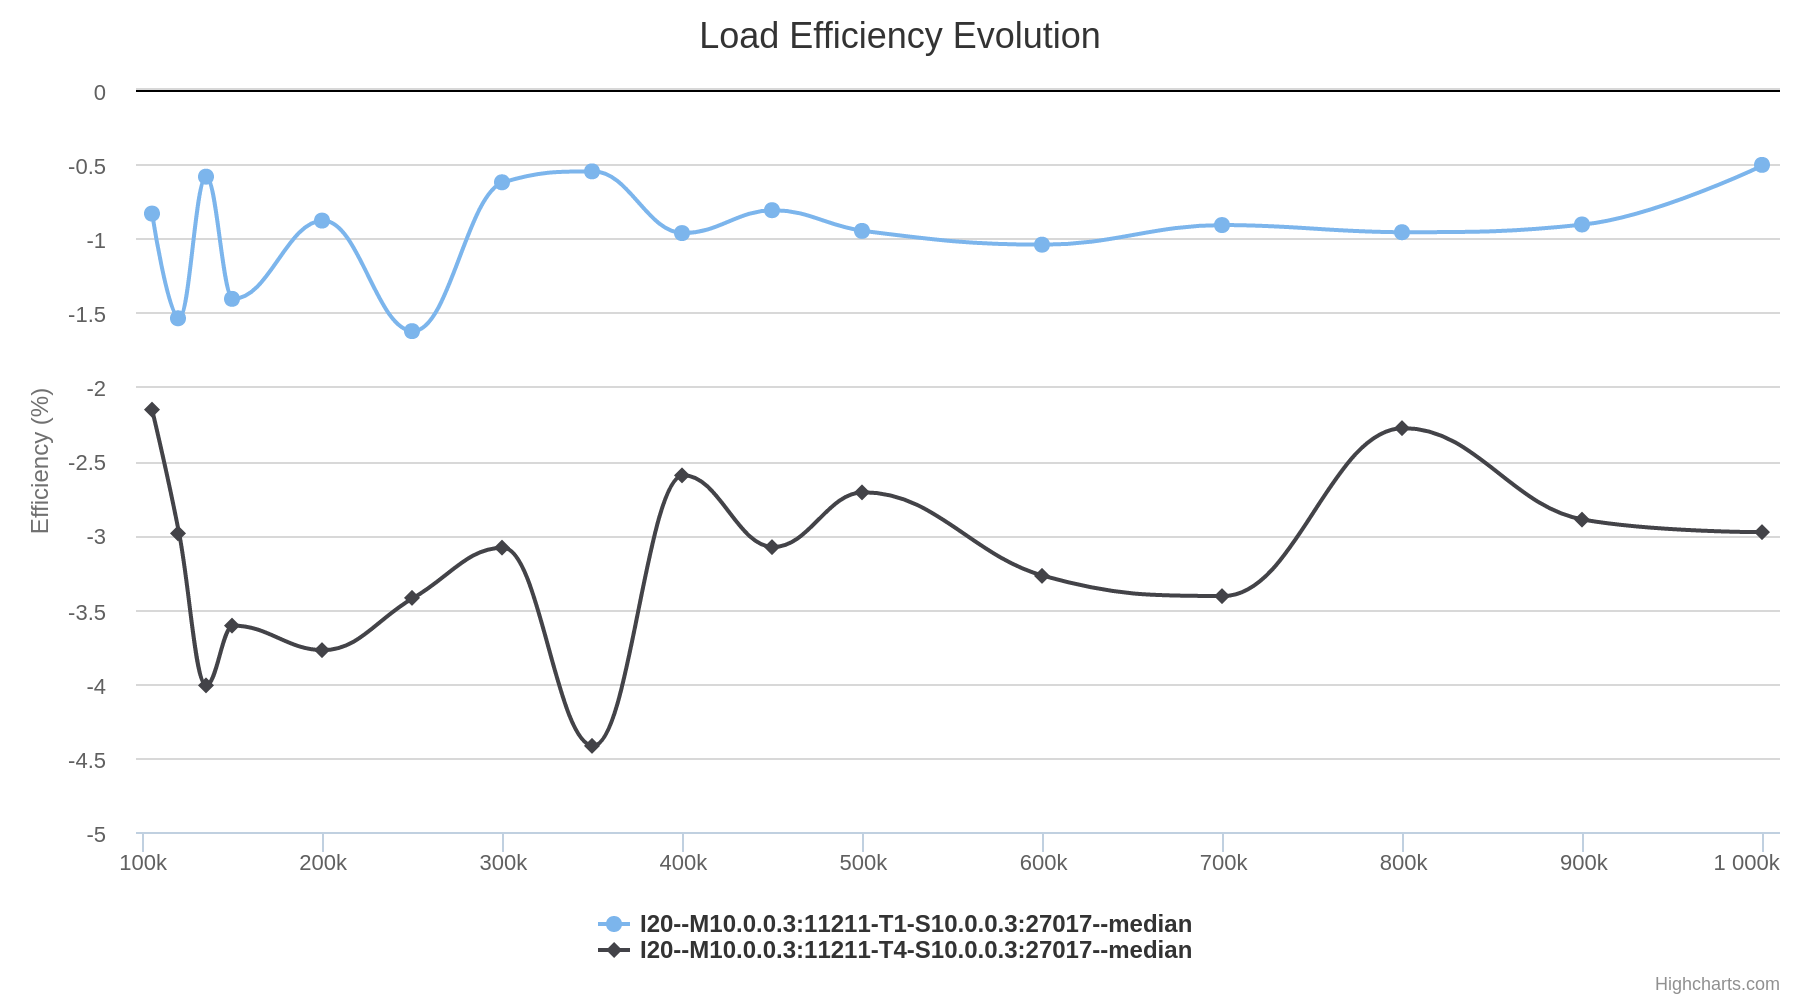
\includegraphics[width=1\linewidth]{images/evaluation/thread-SMremote-load.png}
\caption{Influence of our measurement type on the efficiency regarding client thread number: LOAD phase.}
\label{thread-SMremote-load}
\end{center}
\end{figure}

\begin{figure}[ht]
\begin{center}
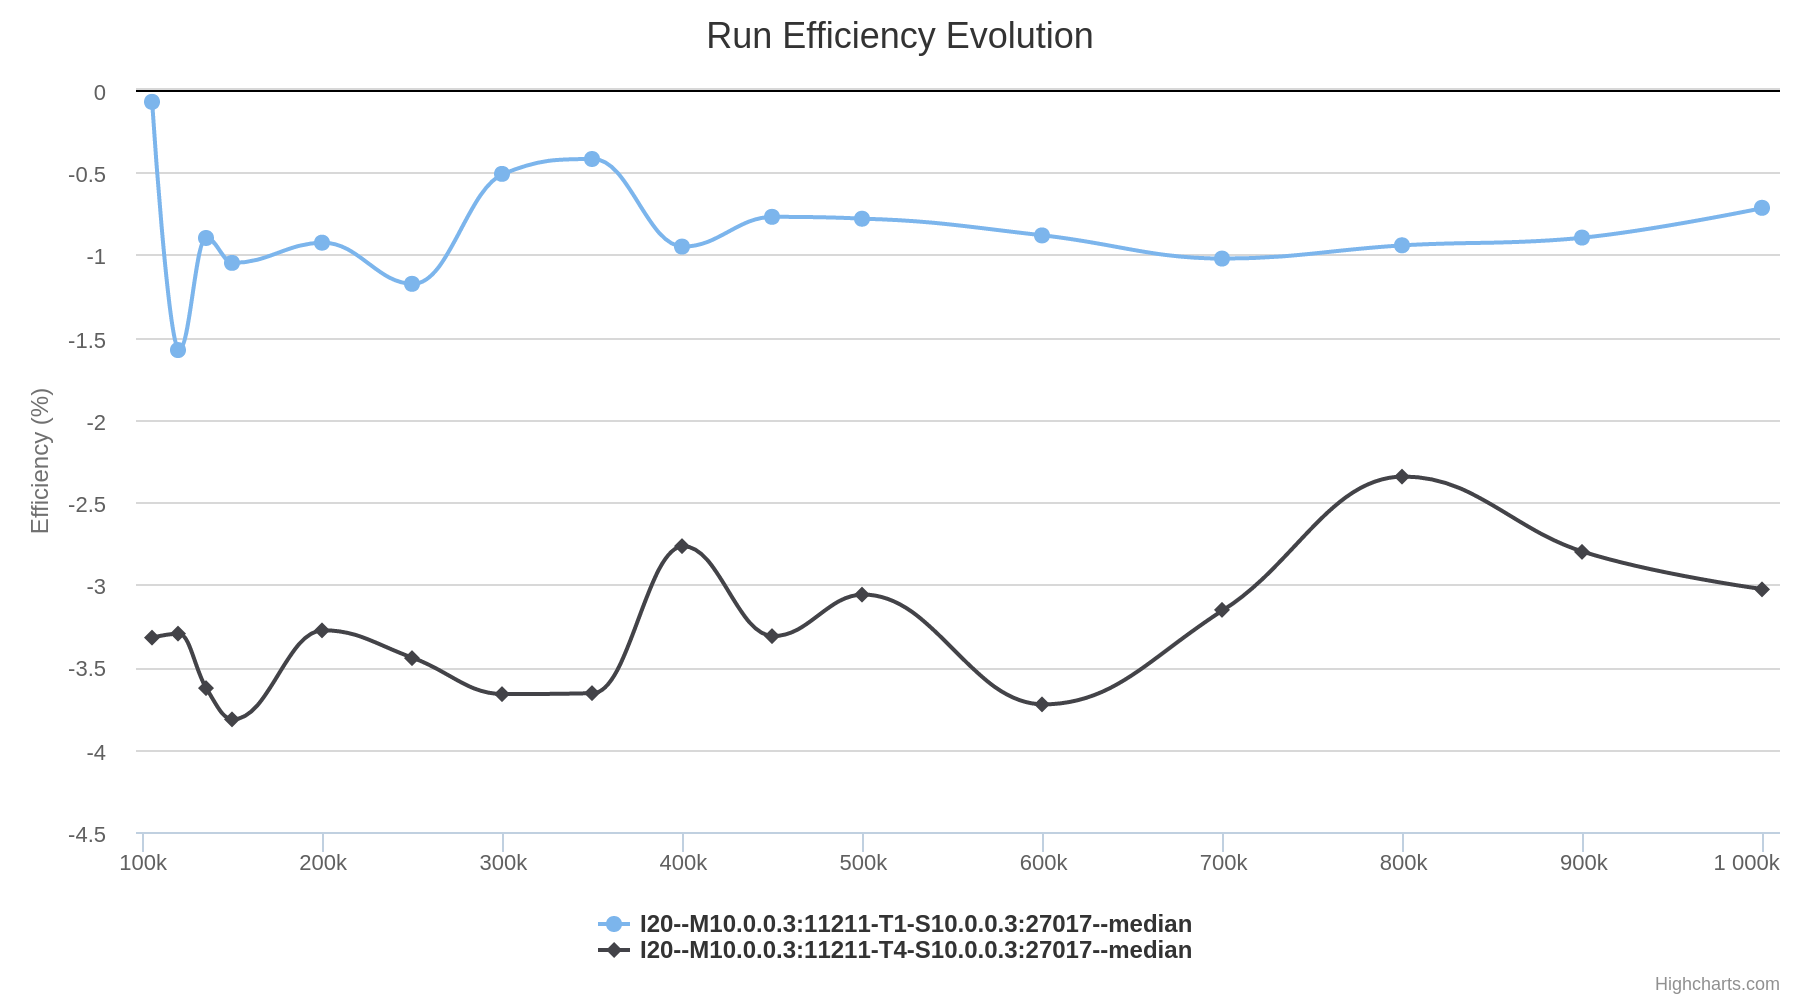
\includegraphics[width=1\linewidth]{images/evaluation/thread-SMremote-run.png}
\caption{Influence of our measurement type on the efficiency regarding client thread number: RUN phase.}
\label{thread-SMremote-run}
\end{center}
\end{figure}

\begin{table}[ht]
\begin{center}
	\begin{tabular}{|c|c|c|}
		\hline
		  & 1 Client Threads DB & 4 Client Threads \\
		\hline
	   	LOAD phase & 0.5\% - 1.5\% slower & 2\% - 4.5\% slower \\
	   	RUN phase & 0\% - 1.5\% slower & 2.3\% - 3.8\% slower \\
	    \hline
	\end{tabular}
	\caption{Influence of the measurement type on the efficiency regarding client thread number.}
\label{thread-table}
\end{center}
\end{table}

The behavior for 10, 20 or even 30 threads is quite different. The more client threads the more dispersion we observe in results. This dispersion is not always negative as for 30 threads in Figure \ref{thread30-SMremote-load} and \ref{thread30-SMremote-run} but still quite unpredictable. This figures have been obtained after $25*2$ iterations.

\begin{figure}[ht]
\begin{center}
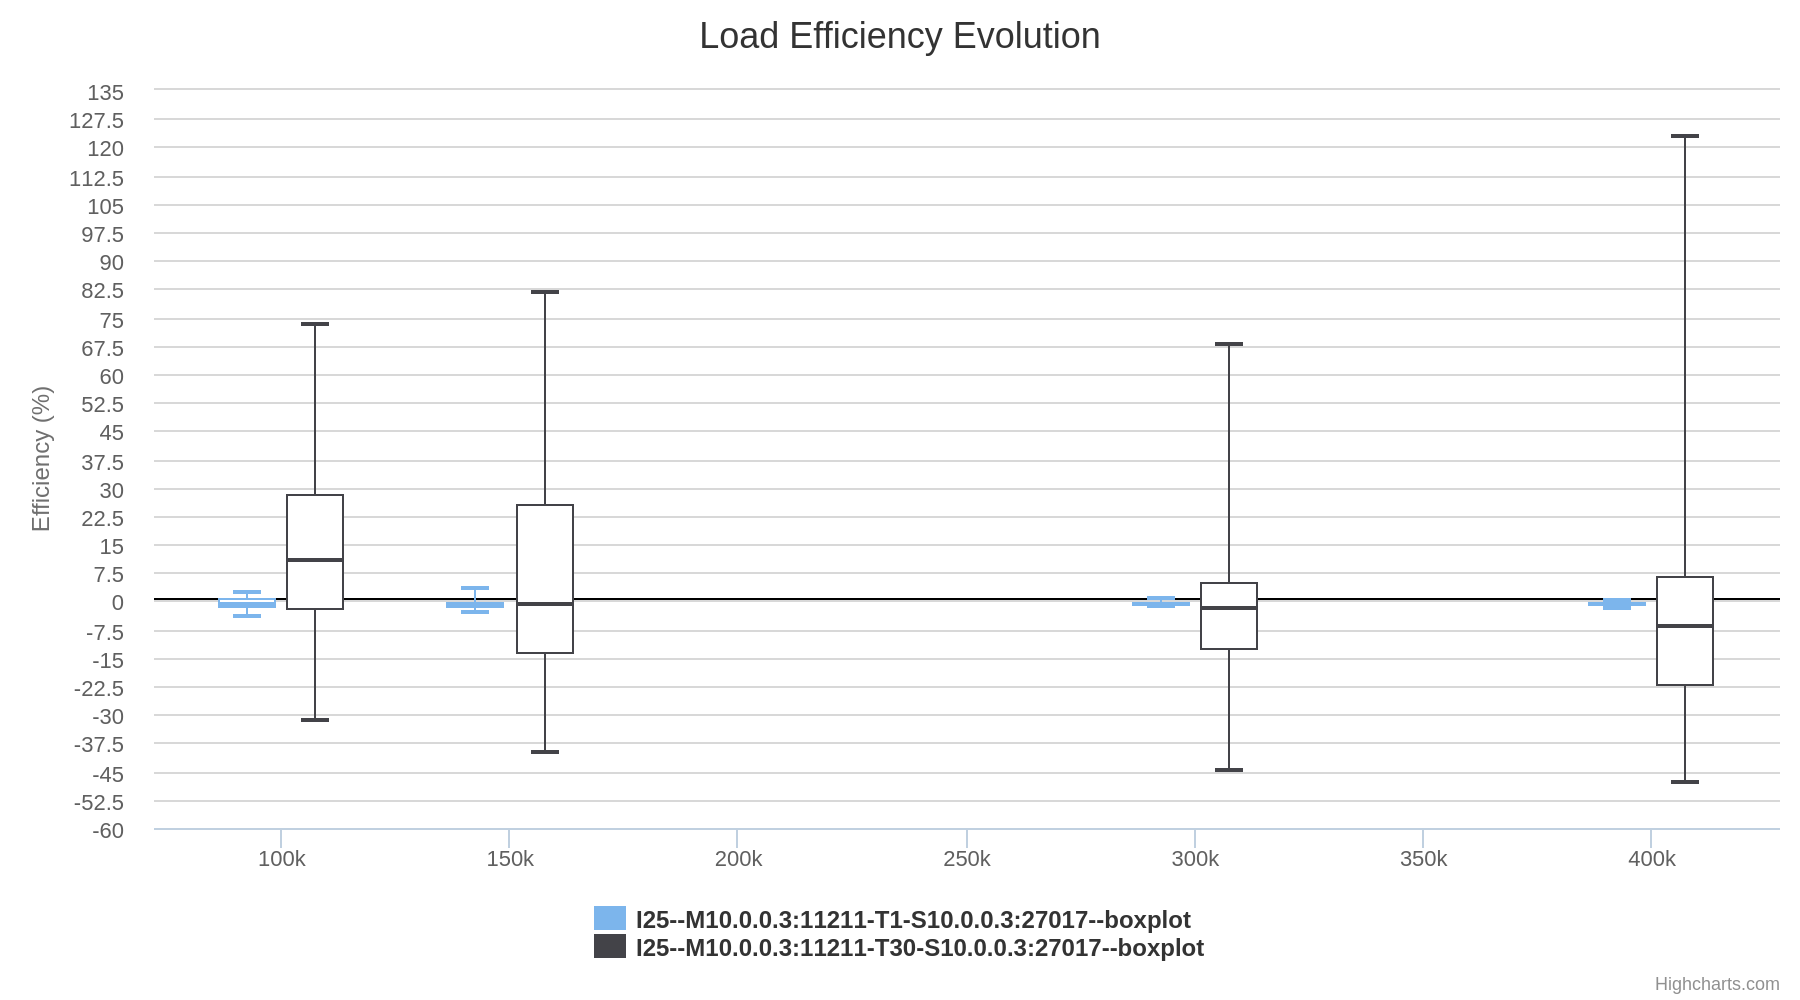
\includegraphics[width=1\linewidth]{images/evaluation/thread30-SMremote-load.png}
\caption{One and thirty client threads dispersion comparison: LOAD phase.}
\label{thread30-SMremote-load}
\end{center}
\end{figure}

\begin{figure}[ht]
\begin{center}
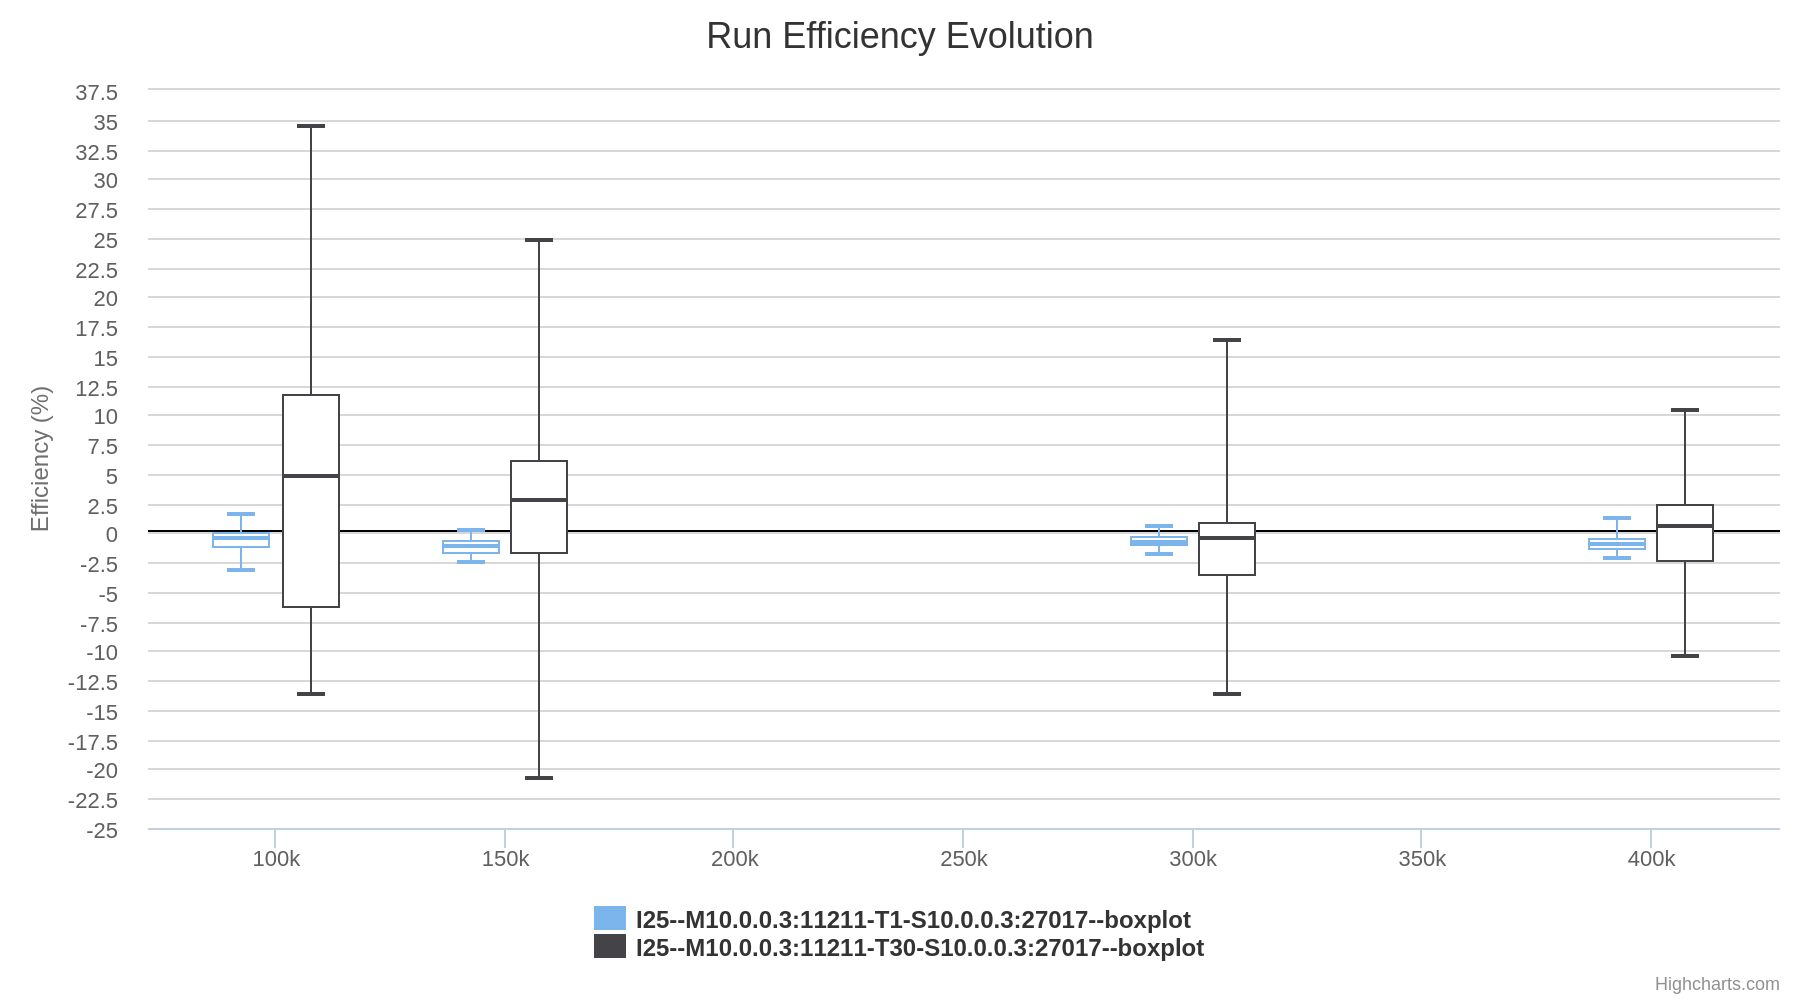
\includegraphics[width=1\linewidth]{images/evaluation/thread30-SMremote-run.png}
\caption{One and thirty client threads dispersion comparison: RUN phase.}
\label{thread30-SMremote-run}
\end{center}
\end{figure}

\paragraph{Conclusion} Our measurement type will influence more YCBS efficiency in a multi threaded environment than in a single threaded environment. \textit{BE CAREFUL: this does not mean that a multi threaded environment is less efficient}, in fact this is a YCSB problem, here, we compare the \textit{influence} of our measurement in both configurations. 

For example, let's say that using RAW measurement type with a single thread and multiple threads  we achieve respectively 5000 and 7000 throughputs and using our measurement type with a single thread and multiple threads we achieve respectively 4500 and 5000 throughputs --- these numbers are for the sake of the example and do not refer to actual values. We have a better efficiency when using multiple client threads BUT our measurement type has a huge influence on the multi threaded environment reducing by 2000 throughputs against 500 for the single threaded environment.

As stated before, our measurement type is using another thread to store measures. Threads should have some OS conflict that slows down the entire process --- context switches, data lookups between threads. The more threads, the more potential conflicts you have, that is why we observe this dispersion. This unpredictable conflicts should also be the source of the larger fluctuations of the multi threaded environment line.
Moreover, measure function in YCSB is synchronized and our measurement type has a little bit more operation to do in this function --- we instantiate our BSON Document there --- thus threads are hanging for more time and this must decreasing the overall efficiency of our measurement type.

\clearpage

\subsubsection{Global tendency by number of points}

As intended, the more points the benchmark has, the closer the execution time of our module is close to the original one in most cases. Indeed, this difference comes from the storage database connection initialization, executor thread creation and the last points fetch at the end. 

\bigskip

A local benchmarked database is drastically reducing performance --- see \ref{memcached_evaluation} --- thus we chose not to compare results with local benchmarked database. Moreover, a local benchmarked database is a rare YCSB user case. We can see on Figures \ref{global-withoutMlocal-load} \&  \ref{global-withoutMlocal-run} the global tendency of our extension module.

Using medians of 20 iterations in the range from 15k points benchmark to 1M points benchmark we are :

\begin{itemize}
\item
never under 6\% slower for the both LOAD and RUN phase
\item
never under 1\% slower for the both LOAD and RUN phase with remote storage (most common use case)
\end{itemize}

Using minimum values of 20 iterations in the range from 30k points benchmark to 1M points benchmark we are :

\begin{itemize}
\item
never under 10\% slower for the LOAD phase
\item
never under 12\% slower for the RUN phase
\end{itemize}

\begin{figure}[ht]
\begin{center}
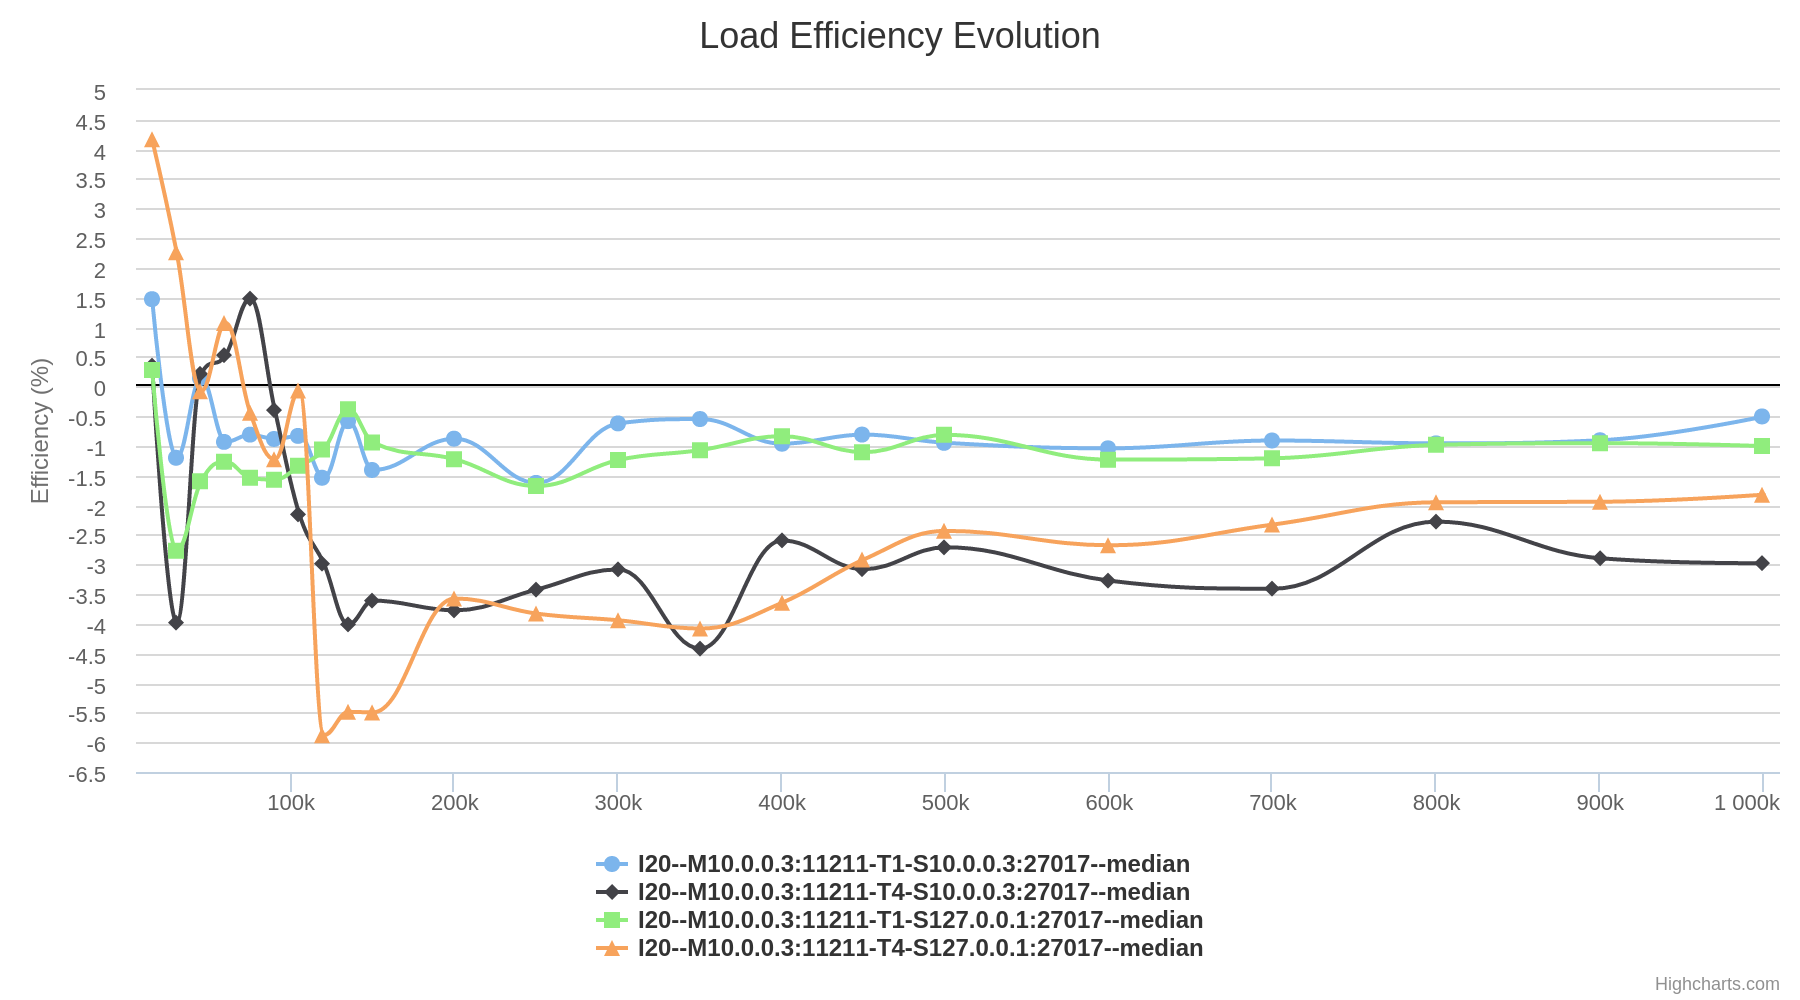
\includegraphics[width=1\linewidth]{images/evaluation/global-withoutMlocal-load.png}
\caption{Global tendency: LOAD phase median.}
\label{global-withoutMlocal-load}
\end{center}
\end{figure}

\begin{figure}[ht]
\begin{center}
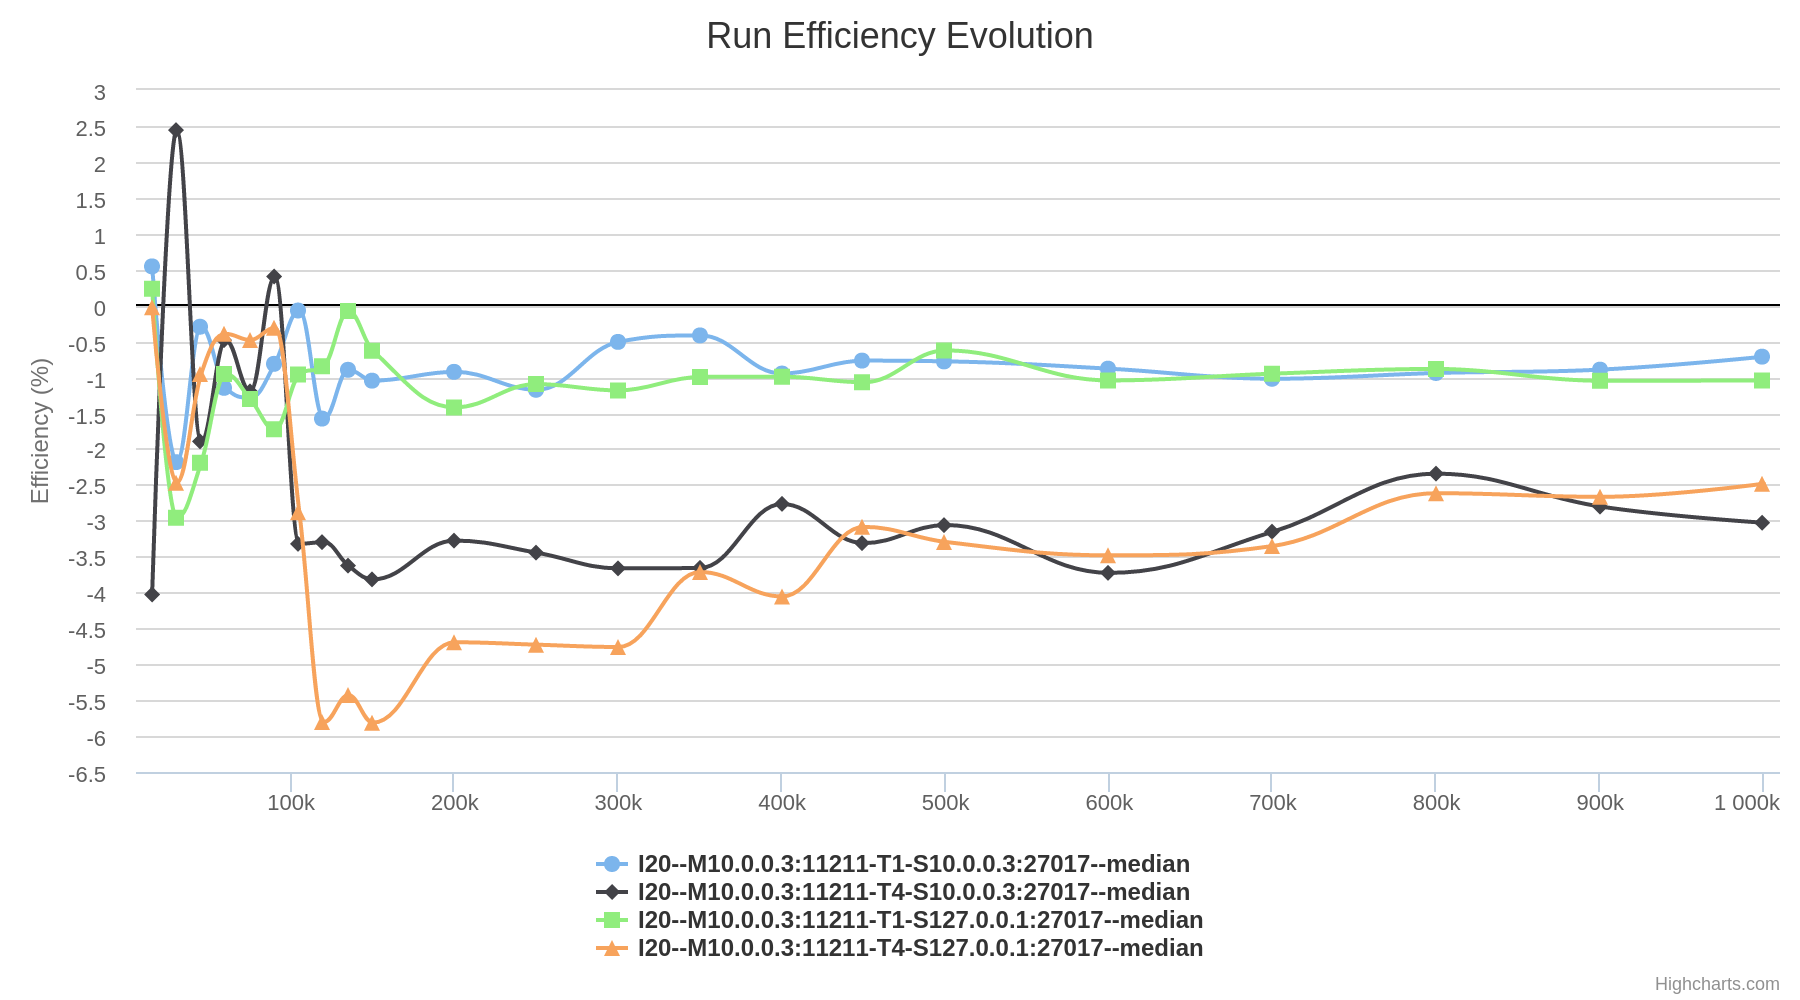
\includegraphics[width=1\linewidth]{images/evaluation/global-withoutMlocal-run.png}
\caption{Global tendency: RUN phase median.}
\label{global-withoutMlocal-run}
\end{center}
\end{figure}

\clearpage

\subsection{Execution time efficiency}

The following Figure \ref{execution_time} has been drawn after $20*2$ iterations of couple of load and run phases --- 20 iterations with the custom measurement type and 20 with the RAW measurement type.

\paragraph{Fixed parameters}
\begin{itemize}
\item
Remote benchmarked database
\item
Remote storage database
\item
single threaded environment (1 client thread)
\end{itemize}

\paragraph{Results}

The execution time efficiency is quasi identical when we tweak parameters like client thread number and local/remote storage database. As you can see on Figure \ref{execution_time}, we are around 7.5 times \textbf{slower} than YCSB on a 1k points benchmark and this is decreasing and then stabilizing around 45k to reach the same execution time as the RAW measurement type.

\begin{figure}[ht]
\begin{center}
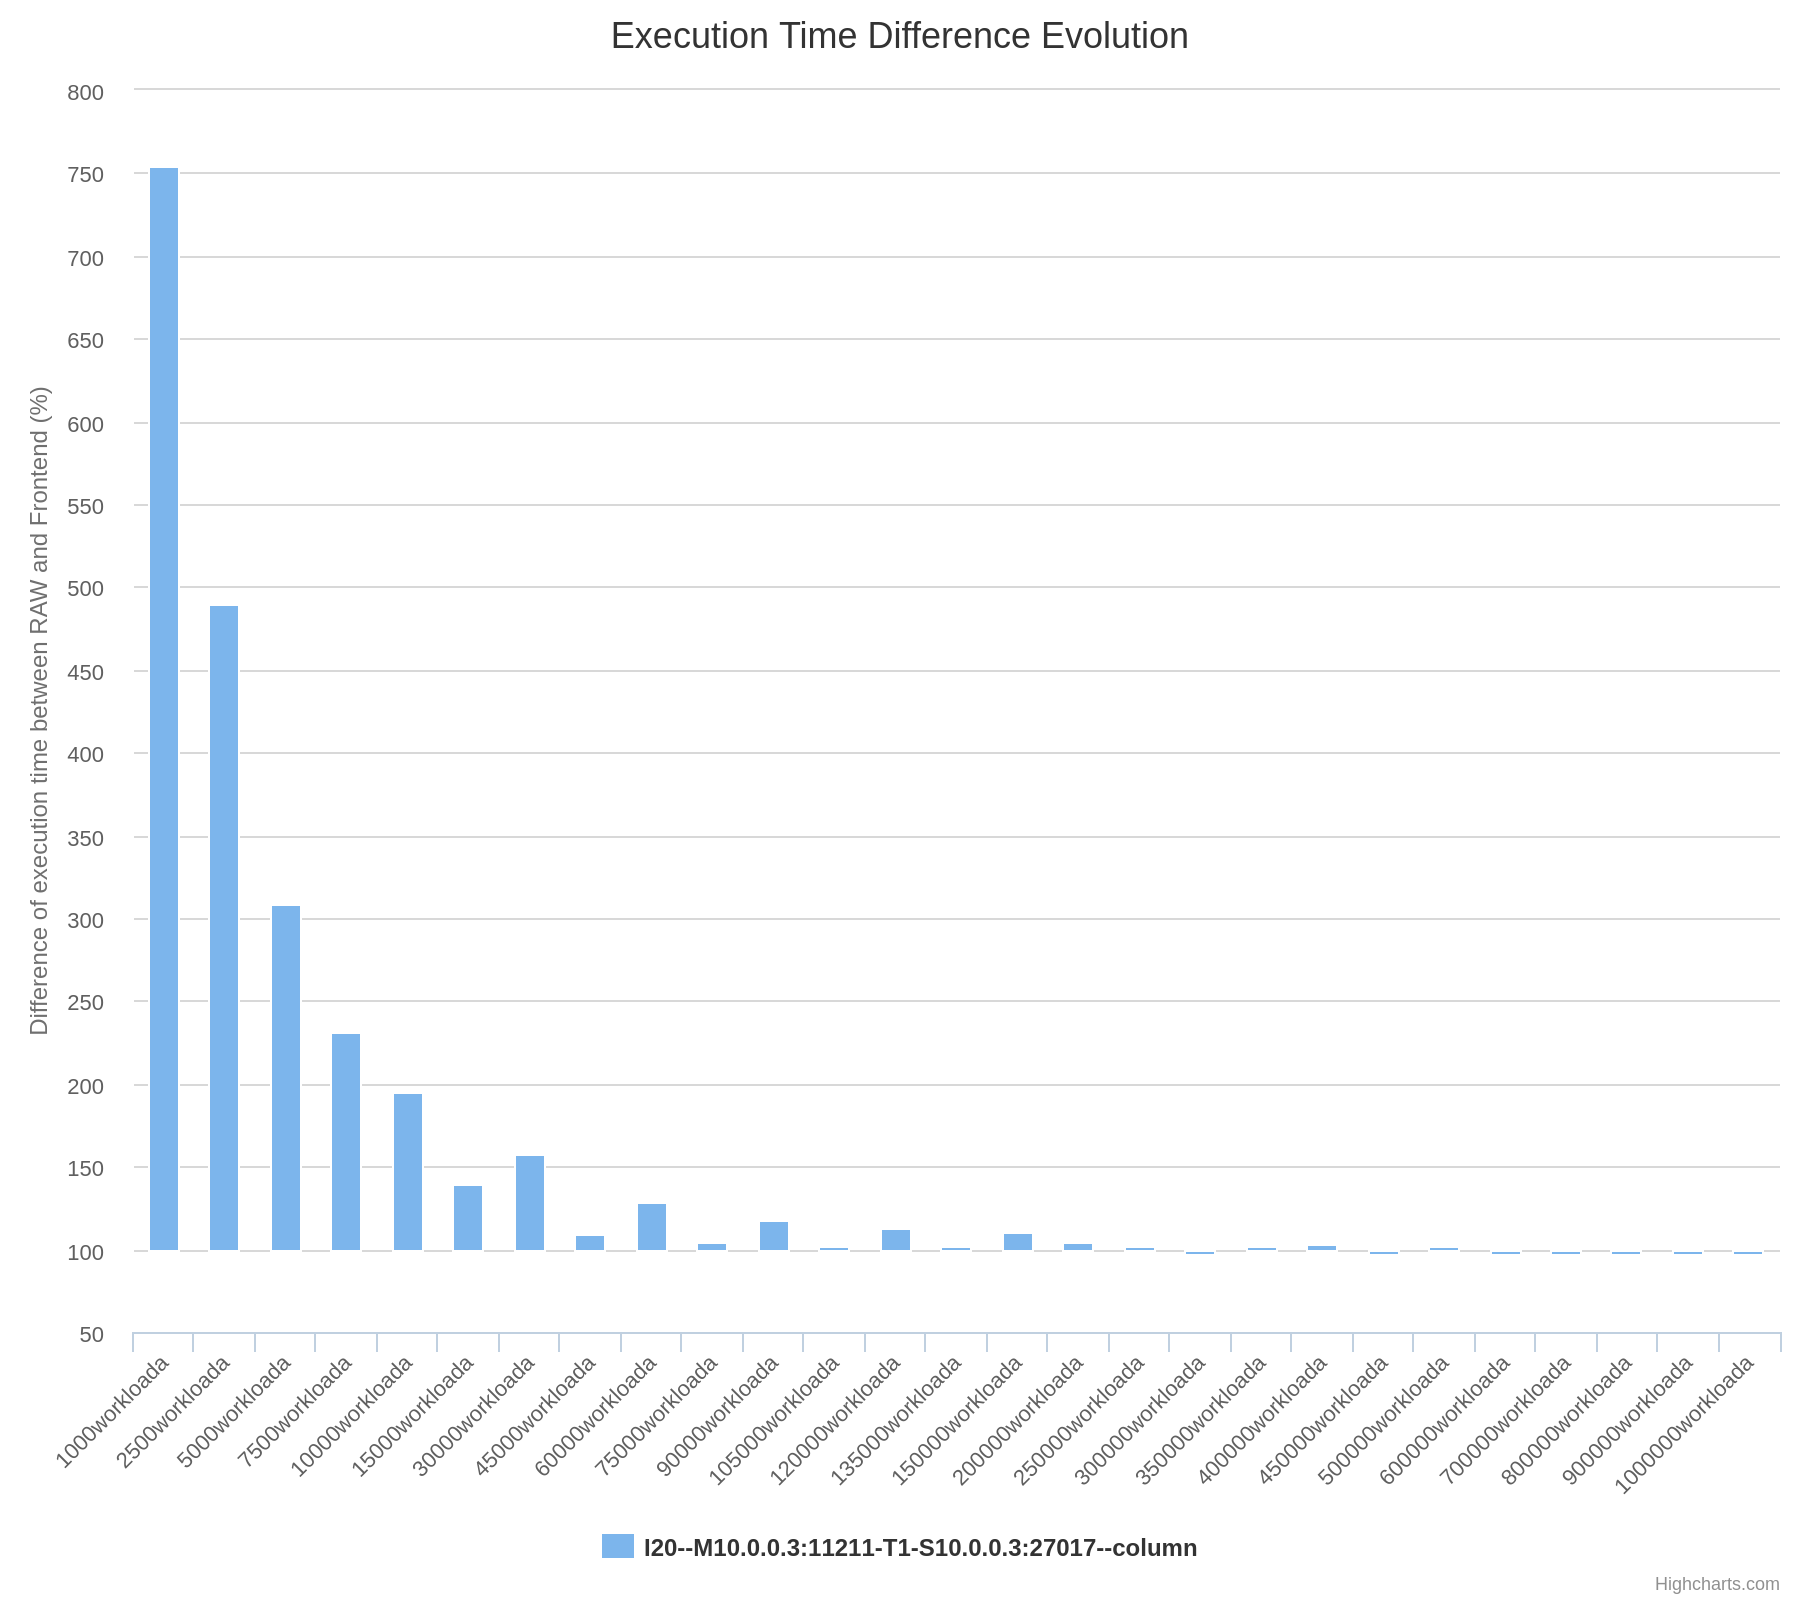
\includegraphics[width=1\linewidth]{images/evaluation/execution_time.png}
\caption{Execution time efficiency evolution comparison chart.}
\label{execution_time}
\end{center}
\end{figure}

\paragraph{Conclusion}

As intended, the more points the benchmark has, the closer the execution time of our module is close to the original one. Indeed, this difference comes from the storage database connection initialization, executor thread creation and the last points fetch process at the end.

\clearpage

\section{Limitations}

\subsection{YCSB extension module}

\subsubsection{Benchmarked database}

The storage process, as it is implemented, should work regardless of the benchmarked database thus you can also use your custom adapters.
However, for now, it has been tested with memcached only.

\subsection{Web visualizer}

\subsubsection{Highcharts}

Highcharts library is a proprietary software, it is allowed to use it for a personal website, a school site or a non-profit organisation which suited our case. However, it is a strong limitation for our application users. 

As charts are handled by an AngularJS directive, we could plug another chart library by creating another directive to overcome this limitation. This new library would need functions to create, delete or modify series after a chart generation in order to work with our implementation.

\subsubsection{Aggregation requests}

Our visualizer will work regardless of the number of points the benchmark has. However, our NodeJS server would be very slow at serving point when dealing with millions of points. Indeed, here a few figures, aggregation requests take around:
\begin{itemize}
\item
20 seconds for a 2 million points to complete on a remote server --- Intel(R) Core(TM) i3-2130 CPU @ 3.40GHz with 8GB of RAM with a 100Mbps connexion
\item
30 seconds for a 10 million points to complete on a local server --- Intel(R) Core(TM) i5-4590 CPU @ 3.30GHz with 32GB of RAM
\end{itemize}

\subsubsection{Storage database}

You could rebuild the entire NodeJS MongoDB API to make it work with another DB but it wasn't our goal to achieve this compatibility.

However, you could use our import module if you really don't want to deal with MongoDB database.

\subsubsection{Display: linear loss of accuracy}

As we see in \ref{server:handling_large_dataset}, our application uses an aggregating process to handle millions of values. This aggregation process is reducing the precision of our displayed charts.

The precision reduction grow linearly when the number of points in your benchmark is increasing. The coefficient of this linear reduction is the constant the user sets based on his computer performances --- the better your machine is, the higher points you can display\footnote{Please consult the README.md file of the visualization application for more information}. 

We have then the following trivial equation where: 
\begin{itemize}
\item
$benchmarkLength$ is the number of points in the benchmark
\item
$fixedUserConstant$ is the constant set by the user in application parameter based on his computer performance
\item
$bucketSize$ is the size of the aggregation buckets --- the higher they are, the lower is the precision as the average is based on more points
\end{itemize}

$$ benchmarkLength = fixedUserConstant * bucketSize $$
$$\Longleftrightarrow bucketSize = \frac{benchmarkLength}{fixedUserConstant} $$

\clearpage

\chapter*{Conclusion}

This internship was for me the first time that I had a real dataset size concerns. Optimizing code and building our solution around these issues were the most interesting parts of this project. Every single mechanism could become a bottleneck when dealing with this amount of data, database aggregation, HTTP communications, Angular page rendering, etc. I regret not to have time to go further on the optimization of the communications between NodeJS and AngularJS with binary compressed data transfer for example but for most of the use cases it would have been "overkill".

Speaking of optimization, the hardest part was to know where to stop. Indeed, each optimization must be done after answering the following question: \textit{"Isn't it too much?"}. When I was trying to redesign some of my module to make it fit the size issue, I tend to try all kind of optimizations I could think of. It was obviously a mistake but fortunately I realized it soon enough. This internship help me understand the basis of how to evaluate the value of an optimization.

The journey abroad reinforce my will to deal with large scale application in depth thus with "Ingénierie du Cloud Computing" option at the EISTI. I wish to discover more of the company's life and working methods on my next internship.

\clearpage

\bibliographystyle{ieeetr}
\bibliography{report}

\clearpage

\includepdf[pages=-, offset=75 -75]{images/cv.pdf}

\newpage

% ==============================================================================
\end{document}
% ==============================================================================